%DIF 1d1
%DIF LATEXDIFF DIFFERENCE FILE
%DIF DEL draft_V2.tex   Mon Apr 19 22:07:25 2021
%DIF ADD main.tex       Mon Apr 19 22:48:58 2021
%DIF < 
%DIF -------
\documentclass[draft,linenumbers]{agujournal2019}

\usepackage{url} 
\usepackage{lineno}
% \usepackage[inline]{trackchanges} 
\usepackage{soul}
\usepackage{natbib}
\usepackage{float}

%\draftfalse

\journalname{JGR Oceans}

%%%%%%%%%%%%%%%%%%%%%%%%%%%%%%%%%%%

%% MACROS
\newcommand{\MKE}{\overline{\textrm{KE}}}
\newcommand{\mKE}{\textrm{MKE}}
\newcommand{\KE}{\textrm{KE}}
\newcommand{\MEKE}{\overline{\textrm{EKE}}}
\newcommand{\EKE}{\textrm{EKE}}
\newcommand{\MCEKE}{\overline{\textrm{CEKE}}}
\newcommand{\CEKE}{\textrm{CEKE}}
\newcommand{\MnCEKE}{\overline{\textrm{nCEKE}}}
\newcommand{\nCEKE}{\textrm{nCEKE}}
\newcommand{\cEddy}{\textrm{cEddy}}
%DIF PREAMBLE EXTENSION ADDED BY LATEXDIFF
%DIF UNDERLINE PREAMBLE %DIF PREAMBLE
\RequirePackage[normalem]{ulem} %DIF PREAMBLE
\RequirePackage{color}\definecolor{RED}{rgb}{1,0,0}\definecolor{BLUE}{rgb}{0,0,1} %DIF PREAMBLE
\providecommand{\DIFadd}[1]{{\protect\color{blue}\uwave{#1}}} %DIF PREAMBLE
\providecommand{\DIFdel}[1]{{\protect\color{red}\sout{#1}}}                      %DIF PREAMBLE
%DIF SAFE PREAMBLE %DIF PREAMBLE
\providecommand{\DIFaddbegin}{} %DIF PREAMBLE
\providecommand{\DIFaddend}{} %DIF PREAMBLE
\providecommand{\DIFdelbegin}{} %DIF PREAMBLE
\providecommand{\DIFdelend}{} %DIF PREAMBLE
\providecommand{\DIFmodbegin}{} %DIF PREAMBLE
\providecommand{\DIFmodend}{} %DIF PREAMBLE
%DIF FLOATSAFE PREAMBLE %DIF PREAMBLE
\providecommand{\DIFaddFL}[1]{\DIFadd{#1}} %DIF PREAMBLE
\providecommand{\DIFdelFL}[1]{\DIFdel{#1}} %DIF PREAMBLE
\providecommand{\DIFaddbeginFL}{} %DIF PREAMBLE
\providecommand{\DIFaddendFL}{} %DIF PREAMBLE
\providecommand{\DIFdelbeginFL}{} %DIF PREAMBLE
\providecommand{\DIFdelendFL}{} %DIF PREAMBLE
%DIF LISTINGS PREAMBLE %DIF PREAMBLE
\RequirePackage{listings} %DIF PREAMBLE
\RequirePackage{color} %DIF PREAMBLE
\lstdefinelanguage{DIFcode}{ %DIF PREAMBLE
%DIF DIFCODE_UNDERLINE %DIF PREAMBLE
  moredelim=[il][\color{red}\sout]{\%DIF\ <\ }, %DIF PREAMBLE
  moredelim=[il][\color{blue}\uwave]{\%DIF\ >\ } %DIF PREAMBLE
} %DIF PREAMBLE
\lstdefinestyle{DIFverbatimstyle}{ %DIF PREAMBLE
	language=DIFcode, %DIF PREAMBLE
	basicstyle=\ttfamily, %DIF PREAMBLE
	columns=fullflexible, %DIF PREAMBLE
	keepspaces=true %DIF PREAMBLE
} %DIF PREAMBLE
\lstnewenvironment{DIFverbatim}{\lstset{style=DIFverbatimstyle}}{} %DIF PREAMBLE
\lstnewenvironment{DIFverbatim*}{\lstset{style=DIFverbatimstyle,showspaces=true}}{} %DIF PREAMBLE
%DIF END PREAMBLE EXTENSION ADDED BY LATEXDIFF

\begin{document}
%DIF >  \title{Climatology of oceanic coherent eddies}
\title{\DIFdelbegin \DIFdel{Climatology, seasonality, and trends }\DIFdelend \DIFaddbegin \DIFadd{A near-global climatology }\DIFaddend of oceanic coherent eddies}

\authors{Josu\'e Mart\'inez-Moreno\affil{1}, Andrew McC. Hogg\affil{1}, and Matthew H. England\affil{2}}
\affiliation{1}{Research School of Earth Science and ARC Center of Excellence for Climate Extremes, Australian National University, Canberra, Australia}
\affiliation{2}{Climate Change Research Centre (CCRC), UNSW Australia, Sydney NSW, Australia}

\correspondingauthor{Josu\'e Mart\'inez-Moreno}{josue.martinezmoreno@anu.edu.au}

\begin{keypoints}
	\item \DIFdelbegin \DIFdel{Kinetic energy of coherent }\DIFdelend \DIFaddbegin \DIFadd{Coherent }\DIFaddend eddies 
	contain around 50\% of the 
	surface ocean kinetic energy budget.
	\item Seasonal cycle of the number of coherent eddies and 
	coherent eddy amplitude reveal a 3-6 month lag to wind forcing\DIFaddbegin \DIFadd{.
	}\DIFaddend \item \DIFdelbegin \DIFdel{Inverse cascade sets up the seasonal lag of }\DIFdelend \DIFaddbegin \DIFadd{The seasonal lag between }\DIFaddend the number and 
	\DIFaddbegin \DIFadd{the }\DIFaddend amplitude of coherent eddies \DIFaddbegin \DIFadd{suggests a role for the inverse cascade}\DIFaddend .
	% \item The coherent eddy amplitude has increase at 
	% a rate of 3 cm per decade since 1993.
\end{keypoints}


\begin{abstract}
	\DIFdelbegin %DIFDELCMD < 

%DIFDELCMD < 	%%%
\DIFdelend Ocean eddies influence regional and global climate through mixing and transport of heat and properties. 
	One of the most recognizable and ubiquitous feature of oceanic eddies are \DIFaddbegin \DIFadd{coherent }\DIFaddend vortices with spatial scales of tens to hundreds of kilometers, frequently referred as ``mesoscale eddies"\DIFdelbegin \DIFdel{or ``coherent eddies". 
	Coherent }\DIFdelend \DIFaddbegin \DIFadd{. 
	Coherent mesoscale }\DIFaddend eddies are known to transport properties across the ocean and to locally affect near-surface wind, cloud properties and rainfall patterns. Although coherent eddies are ubiquitous, \DIFdelbegin \DIFdel{yet }\DIFdelend their climatology, seasonality and long-term temporal evolution remains poorly understood. 
	\DIFdelbegin \DIFdel{Thus}\DIFdelend \DIFaddbegin \DIFadd{Here}\DIFaddend , we examine the kinetic energy contained by coherent eddies and \DIFdelbegin \DIFdel{we present the annual }\DIFdelend \DIFaddbegin \DIFadd{present the seasonal, inter-annual }\DIFaddend and long-term \DIFdelbegin \DIFdel{changes of automatically identified coherent eddies }\DIFdelend \DIFaddbegin \DIFadd{variability of $\sim$37 million coherent eddies features detected }\DIFaddend from satellite observations \DIFdelbegin \DIFdel{from }\DIFdelend \DIFaddbegin \DIFadd{between }\DIFaddend 1993 to 2019. 
	Around 50\% of the kinetic energy contained by ocean eddies corresponds to coherent eddies. 
	Additionally, a strong \DIFdelbegin \DIFdel{hemispherical }\DIFdelend seasonal cycle is observed, with a 3--6 months lag between the wind forcing and the response of the coherent eddy field. 
	\DIFdelbegin \DIFdel{Furthermore, the }\DIFdelend \DIFaddbegin \DIFadd{The }\DIFaddend seasonality of the number of coherent eddies and their amplitude reveals that the number of coherent eddies responds faster to the forcing ($\sim$3 months), than the coherent eddy amplitude (which is lagged by $\sim$6 months).  
	%DIF < There are regions that show a pronounced influence of coherent eddies, notably, the East Indian Ocean, the East Tropical Pacific Ocean, and the South Atlantic Ocean. 
	%DIF < In these locations, a strong seasonal cycle and interannual variability can be observed in both satellite and numerical models. Although, there is agreement between these products on the seasonality of the number of eddies, the seasonality of the coherent eddy amplitude between these products show some inconsistencies. 
	%DIF < Long-term trends of the coherent eddy amplitude from satellite observations and the state of the art model show significant increases in the eddy amplitude of $\sim$3cm per decade in large portions of the ocean, while the number of coherent eddies remains constant. 
	\DIFaddbegin \DIFadd{This seasonal cycle of the coherent eddy properties is spatially variable, thus we also analyze the coherent eddy climatology in key oceanic regions.
	}\DIFaddend Our analysis highlights the relative importance of the coherent eddy field in the ocean kinetic energy budget, implies a strong response of the eddy number and eddy amplitude to forcing at different time-scales, and showcases the seasonality, and multidecadal trends of coherent eddy properties. 

	\noindent\textbf{Plain language summary}

	Coherent eddies are the most common feature \DIFdelbegin \DIFdel{in the oceans }\DIFdelend \DIFaddbegin \DIFadd{of ocean variability }\DIFaddend observable from satellites. They are crucial in ocean dynamics as they can transport  properties over long distances and interact with the atmosphere. Our study investigates the seasonal\DIFaddbegin \DIFadd{, interannual, }\DIFaddend and long-term changes in the abundance and intensity of coherent eddies, by automatically identifying individual eddies over the \DIFaddbegin \DIFadd{available }\DIFaddend satellite altimeter record. The seasonal cycle suggests a transition from numerous, smaller, and weaker coherent eddies, to fewer and larger, and stronger coherent eddies over the season. In addition, a long-term adjustment of the coherent eddy field is identified \DIFdelbegin \DIFdel{possible due }\DIFdelend \DIFaddbegin \DIFadd{with possible links }\DIFaddend to long-term changes in the climate system.

\end{abstract}	

\section{Introduction}

Mesoscale ocean variability with spatial scales of tens to hundreds of kilometers is comprised of processes such as vortices, waves, and jets \citep{Ferrari_energy_2009, Fu_Eddy_2010}. 
These mesoscale processes are highly energetic, and they play a crucial role in the transport of heat, salt, momentum, and other tracers through the ocean \citep{Wunsch_energetics_2004, Wyrtki_Eddy_1976, Gill_Energy_1974}. \DIFdelbegin \DIFdel{Possibly, }\DIFdelend \DIFaddbegin \DIFadd{One of }\DIFaddend the most recognizable and abundant \DIFdelbegin \DIFdel{process observed from satellites is }\DIFdelend \DIFaddbegin \DIFadd{ocean processes observable from space are }\DIFaddend mesoscale vortices. Although mesoscale vortices are commonly referred to in \DIFaddbegin \DIFadd{the }\DIFaddend literature as ``mesoscale eddies", this term is also often used to describe the total mesoscale ocean variability (the time-varying component of the mesoscale flow), thus, \DIFdelbegin \DIFdel{here }\DIFdelend \DIFaddbegin \DIFadd{to avoid ambiguity }\DIFaddend we will refer to mesoscale vortices as \emph{coherent eddies}. \DIFaddbegin \DIFadd{Coherent eddies are abundant and energetic; therefore they are also essential to ocean dynamics as concluded by many previous studies \mbox{%DIFAUXCMD
\citep{Hogg_Interdecadal_2006,Siegel_Bio_2011,BeronVera_Agulhas_2013,Frenger_Imprint_2013,Frenger_Southern_2015,Pilo_eddy_2015,Schubert_submesoscale_2019,Patel_SO_eddies_2020}}\hspace{0pt}%DIFAUXCMD
.
}\DIFaddend 



Coherent eddies are quasi-circular \DIFaddbegin \DIFadd{geostrophic }\DIFaddend currents. According to their rotational direction \DIFaddbegin \DIFadd{and the sign of the Coriolis parameter}\DIFaddend , the sea surface height anomaly within a coherent eddy can have a negative or positive sea surface height anomaly (cold-core and warm-core coherent eddies, respectively). 
This characteristic sea surface height signature of coherent eddies has been utilized to \DIFdelbegin \DIFdel{automatically }\DIFdelend identify and track coherent eddies from satellite altimetry \DIFdelbegin \DIFdel{\mbox{%DIFAUXCMD
\citep{Cui_eddy_identification_2020,Martinez_TKE_2019, Ashkezari_eddies_2016, Faghmous_A_2015,Chelton_Global_2007}}\hspace{0pt}%DIFAUXCMD
.}\DIFdelend \DIFaddbegin \DIFadd{(e.g., \mbox{%DIFAUXCMD
\citealp{Chelton_Global_2007, Faghmous_A_2015, Ashkezari_eddies_2016,Martinez_TKE_2019, Cui_eddy_identification_2020}}\hspace{0pt}%DIFAUXCMD
). 
}\DIFaddend Automated identification algorithms of coherent eddies have \DIFdelbegin \DIFdel{shown }\DIFdelend \DIFaddbegin \DIFadd{revealed }\DIFaddend their ubiquity in the oceans, with a predominant influence at \DIFdelbegin \DIFdel{hotpots }\DIFdelend \DIFaddbegin \DIFadd{hotspots }\DIFaddend of eddy activity such as \DIFdelbegin \DIFdel{boundary }\DIFdelend \DIFaddbegin \DIFadd{in boundary current }\DIFaddend extensions and the Antarctic Circumpolar Current. In these regions, \DIFdelbegin \DIFdel{\mbox{%DIFAUXCMD
\citet{Chelton_The_2011} }\hspace{0pt}%DIFAUXCMD
}\DIFdelend \DIFaddbegin \DIFadd{it has been }\DIFaddend estimated that coherent eddies contribute around 40--50\% of the \DIFaddbegin \DIFadd{net }\DIFaddend mesoscale kinetic energy \citep{Chelton_The_2011} and thus a significant fraction of the total kinetic energy \citep{Ferrari_energy_2009}. 
Although this \DIFdelbegin \DIFdel{unique }\DIFdelend estimate showcases the importance of the mesoscale coherent eddy field, the energy contained by coherent eddies was estimated by extracting the \DIFdelbegin \DIFdel{geostrophic velocities within the detected coherent eddies, thus}\DIFdelend \DIFaddbegin \DIFadd{total geostrophic velocity within the radius of each detected coherent eddy; thus, }\DIFaddend it is possible \DIFdelbegin \DIFdel{it }\DIFdelend \DIFaddbegin \DIFadd{that this estimate }\DIFaddend may contain energy from other processes. 
\DIFdelbegin \DIFdel{Coherent eddies are not only abundant and may have a large proportion of the surface kinetic energy budget, but they are also essential to ocean dynamics as concluded by many previous studies \mbox{%DIFAUXCMD
\citep{Patel_SO_eddies_2020,Schubert_submesoscale_2019,Pilo_eddy_2015,Frenger_Southern_2015,Frenger_Imprint_2013,BeronVera_Agulhas_2013,Siegel_Bio_2011,Hogg_Interdecadal_2006}}\hspace{0pt}%DIFAUXCMD
}\DIFdelend \DIFaddbegin \DIFadd{Here we extend on this past work by reconstructing the surface imprint of coherent eddies using a new eddy tracking algorithm and using the latest  available satellite record}\DIFaddend .


There is broad consensus that mesoscale eddy kinetic energy has a pronounced seasonal variability \DIFdelbegin \DIFdel{\mbox{%DIFAUXCMD
\citep{Uchida_Seasonality_2017,Kang_On_2017,Qiu_seasonal_2004, Qiu_seasonal_1999}}\hspace{0pt}%DIFAUXCMD
}\DIFdelend \DIFaddbegin \DIFadd{\mbox{%DIFAUXCMD
\citep{Qiu_seasonal_1999,Qiu_seasonal_2004,Kang_On_2017,Uchida_Seasonality_2017}}\hspace{0pt}%DIFAUXCMD
}\DIFaddend . 
Several hypotheses have been proposed to explain this seasonality including: seasonal variations of atmospheric forcing \citep{Sasaki_seasonal_2014}, seasonality of the mixed layer depth \citep{Qiu_seasonal_2014,Callies_season_2015}, seasonality of the intensity of barotropic instability \citep{Qiu_seasonal_2004}, the variability of the baroclinic instability due to the seasonality of the vertical shear \citep{Qiu_seasonal_1999}, and a seasonal lag of the inverse energy cascade (i.e. energy is transported between scales, from small to large; \citealp{Arbic_cascade_2013}) in combination with the presence of a front in the mixed layer, which can lead to a seasonal cycle of the baroclinic instability \citep{Qiu_seasonal_2014}. On one hand, processes such as barotropic and baroclinic instabilities control the seasonality of coherent eddies in the ocean. 
On the other hand, recent studies using observations and eddy-permitting climate models suggest several long-term adjustments of the global ocean capable of long-term changes in the coherent eddy field. 
Such readjustments include a multidecadal increase in the ocean stratification \DIFdelbegin \DIFdel{resulted }\DIFdelend \DIFaddbegin \DIFadd{resulting }\DIFaddend from temperature and salinity changes \citep{Li_stratification_2020}, a horizontal \DIFdelbegin \DIFdel{readjusment of the }\DIFdelend \DIFaddbegin \DIFadd{readjustment of }\DIFaddend sea surface temperature gradients \DIFdelbegin \DIFdel{\mbox{%DIFAUXCMD
\citep{Ruela_SST_trends_2020,Bouali_SST_grad_trends_2017,Cane_sst_trends_1997}}\hspace{0pt}%DIFAUXCMD
}\DIFdelend \DIFaddbegin \DIFadd{\mbox{%DIFAUXCMD
\citep{Cane_sst_trends_1997,Bouali_SST_grad_trends_2017,Ruela_SST_trends_2020}}\hspace{0pt}%DIFAUXCMD
}\DIFaddend , and an intensification of the kinetic energy, eddy kinetic energy, and mesoscale eddy kinetic energy over the last 3 decades as a consequence of an increase in wind forcing \citep{Hu_acceleration_2020,Wunsch_speeding_2020,Martinez_Kinetic_2021}. 
All these seasonal factors and long-term readjustments directly influence the annual and decadal response of the coherent eddy field, however, the seasonality of the coherent component of the eddy kinetic energy, as well as the seasonal cycle and trends of the coherent eddy statistics\DIFaddbegin \DIFadd{, }\DIFaddend remain unknown.

Here we present a new global climatology of the coherent eddy kinetic energy by reconstructing the coherent eddy signature from satellite observations. Our study documents the seasonal cycle of the coherent eddy kinetic energy, and \DIFaddbegin \DIFadd{the }\DIFaddend seasonal cycle and long-term trends of the coherent eddy properties over the satellite record. 
Moreover, we conduct more \DIFdelbegin \DIFdel{detail analysis }\DIFdelend \DIFaddbegin \DIFadd{detailed analyses }\DIFaddend in regions where coherent eddies dominate the eddy kinetic energy field. 
\DIFdelbegin \DIFdel{This }\DIFdelend \DIFaddbegin \DIFadd{The rest of this }\DIFaddend paper is structured as follows:  the data sources and methodology are described in \DIFdelbegin \DIFdel{section }\DIFdelend \DIFaddbegin \DIFadd{Section }\DIFaddend \ref{sec:Methods}.
Then, we present the climatology, energy ratios, and global seasonality of the coherent eddy kinetic energy in \DIFdelbegin \DIFdel{section }\DIFdelend \DIFaddbegin \DIFadd{Section }\DIFaddend \ref{sec:CEKE_climatology}. 
Section \ref{sec:CE_stats} \DIFdelbegin \DIFdel{presents }\DIFdelend \DIFaddbegin \DIFadd{outlines }\DIFaddend the global climatology and seasonality of coherent eddy properties, followed by long-term changes of the coherent eddy properties (\DIFdelbegin \DIFdel{section }\DIFdelend \DIFaddbegin \DIFadd{Section }\DIFaddend \ref{sec:CE_trends}). Then we focus our attention on the seasonal cycle and coherent eddy properties in regions dominated by coherent eddies (\DIFdelbegin \DIFdel{section }\DIFdelend \DIFaddbegin \DIFadd{Section }\DIFaddend \ref{sec:CE_regional_stats}). 
Finally, \DIFdelbegin \DIFdel{section }\DIFdelend \DIFaddbegin \DIFadd{Section }\DIFaddend \ref{sec:Conclusions} summarizes the main results and discusses the implications of this study.

\section{Methods}
\label{sec:Methods}
	We use daily sea surface height (SSH) data made available by the Copernicus Marine Environment Monitoring Service in near real time \citep{CMEMS_aviso_2017}. 
	This gridded product contains the sea surface height and geostrophic velocities with daily 0.25$^\circ$ resolution from January 1993 to 2019.
	The daily geostrophic velocities \DIFdelbegin \DIFdel{allowed }\DIFdelend \DIFaddbegin \DIFadd{allow }\DIFaddend us to compute the kinetic energy ($\KE$) and eddy kinetic energy ($\EKE$) over the satellite record. The main source of $\EKE$ is the time-varying wind \citep{Ferrari_energy_2009}\DIFdelbegin \DIFdel{, thuswe computed }\DIFdelend \DIFaddbegin \DIFadd{; thus, we also compute }\DIFaddend the seasonal cycle of the wind magnitude from the JRA55 reanalysis \citep{JMA_JRA55_2013} using wind velocities at 10m above the ocean's surface. 

	Over the same record, coherent eddy statistics from \citet{Martinez_TKE_2019}, hereafter \DIFdelbegin \DIFdel{M-M}\DIFdelend \DIFaddbegin \DIFadd{MM19}\DIFaddend , are analyzed and compared \DIFdelbegin \DIFdel{to }\DIFdelend \DIFaddbegin \DIFadd{with }\DIFaddend those released by \citet{Chelton_mesoscale_2013}, \DIFdelbegin \DIFdel{both }\DIFdelend \DIFaddbegin \DIFadd{hereafter CS13. 
	Both }\DIFaddend datasets are gridded in a 1$^\circ$ resolution \DIFdelbegin \DIFdel{. 
	Although both datasets }\DIFdelend \DIFaddbegin \DIFadd{and }\DIFaddend are produced via automated eddy identification algorithms using closed contours of SSH\DIFaddbegin \DIFadd{. However}\DIFaddend , these datasets have important differences in the criteria they use to identify and record coherent eddies statistics. 
	The major differences include\DIFdelbegin \DIFdel{; }\DIFdelend \DIFaddbegin \DIFadd{: }\DIFaddend (i) \DIFdelbegin \DIFdel{M-M}\DIFdelend \DIFaddbegin \DIFadd{MM19}\DIFaddend 's algorithm requires an adjustment between a 2D Gaussian and the SSH anomaly (SSHa) surface within the \DIFdelbegin \DIFdel{identify }\DIFdelend \DIFaddbegin \DIFadd{identified }\DIFaddend closed contour, while \DIFdelbegin \DIFdel{Chelton}\DIFdelend \DIFaddbegin \DIFadd{CS13}\DIFaddend 's only uses the \DIFdelbegin \DIFdel{outer-most }\DIFdelend \DIFaddbegin \DIFadd{outermost }\DIFaddend closed contour of SSH; (ii) \DIFdelbegin \DIFdel{M-M}\DIFdelend \DIFaddbegin \DIFadd{MM19}\DIFaddend 's dataset reports the maximum SSHa within the identified coherent eddy, while \DIFdelbegin \DIFdel{Chelton}\DIFdelend \DIFaddbegin \DIFadd{CS13}\DIFaddend 's algorithm reports the maximum SSH value minus the discrete level in which the coherent eddy was identified; \DIFdelbegin \DIFdel{M-M}\DIFdelend \DIFaddbegin \DIFadd{and (iii) MM19}\DIFaddend 's dataset includes all detected coherent eddies, while \DIFdelbegin \DIFdel{Chelton}\DIFdelend \DIFaddbegin \DIFadd{CS13}\DIFaddend 's dataset excludes \DIFdelbegin \DIFdel{(iii) }\DIFdelend coherent eddies with lifetimes shorter than four weeks and \DIFdelbegin \DIFdel{(iv) }\DIFdelend coherent eddy amplitudes smaller than 1cm. Moreover, \DIFdelbegin \DIFdel{M-M}\DIFdelend \DIFaddbegin \DIFadd{MM19}\DIFaddend 's algorithm allows the reconstruction of the coherent eddy field under the assumption that coherent eddies have a 2D Gaussian imprint in the sea surface height. This Gaussian reconstruction of the coherent eddy field  then \DIFdelbegin \DIFdel{allow }\DIFdelend \DIFaddbegin \DIFadd{allows }\DIFaddend us to estimate the coherent geostrophic eddy velocities and thus the kinetic energy contained only by coherent eddies.

	\subsection{Kinetic Energy decomposition}

	Kinetic energy is commonly divided into the mean and time-varying components through a Reynolds decomposition. At a given time, the surface velocity field $\mathbf{u} = (u,v)$ is split into the time mean ($\mathbf{\overline{u}}$) and time varying components ($\mathbf{u'}$). Moreover, \DIFdelbegin \DIFdel{M-M }\DIFdelend \DIFaddbegin \DIFadd{MM19 }\DIFaddend proposed to further decompose the eddy kinetic energy into the energy contained by coherent features ($\mathbf{u'_e}$) and non-coherent features ($\mathbf{u'_n}$). Therefore the KE equation can be written as:

	\begin{equation}
		\mathrm{KE} = \underbrace{\overline{u}^2 + \overline{v}^2}_{\mKE} + 
		\underbrace{\underbrace{{u'}_e^2+{v'}_e^2}_{\CEKE}  + \underbrace{{u'}_n^2+{v'}_n^2}_{\nCEKE} + \mathcal{O}_c^2 }_{\EKE} + \mathcal{O}^2
	\end{equation}

	Due to the properties of this decomposition, the second order term $\mathcal{O}^2$ is zero when averaged over the same period as $\mathbf{\overline{u}}$. However, $\mathcal{O}_c^2$ is not \DIFdelbegin \DIFdel{necessarly }\DIFdelend \DIFaddbegin \DIFadd{necessarily }\DIFaddend negligible, unless it is averaged over time and space. More information about the decomposition of the field into coherent features and non-coherent features is explained \DIFdelbegin \DIFdel{by }\DIFdelend \DIFaddbegin \DIFadd{in }\DIFaddend \citet{Martinez_TKE_2019}. A global snapshot of each component of kinetic energy decomposition is shown in Figure \ref{fig:eddy_snapshot}, where the $\KE$ and $\EKE$ are comprised of rings and filaments. As expected, the decomposition of $\EKE$ into $\CEKE$ and $\nCEKE$ components \DIFdelbegin \DIFdel{exhibit }\DIFdelend \DIFaddbegin \DIFadd{exhibits }\DIFaddend only ring-like signatures expected of coherent eddies, while the non-coherent component shows \DIFdelbegin \DIFdel{filaments and some miss-identified }\DIFdelend \DIFaddbegin \DIFadd{primarily filaments, with some mis-identified }\DIFaddend coherent eddies.

	\begin{figure}[t]
	    \centering
	    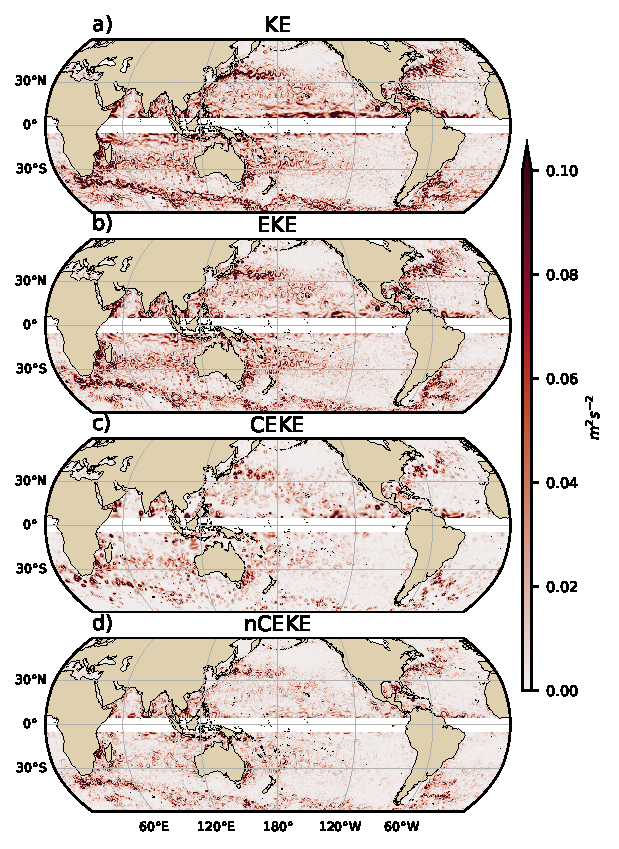
\includegraphics[width=95mm]{figures/snapshot_ke_maps_satellite_large.pdf}
	    \caption{Snapshot of surface kinetic energy ($\MKE$), surface eddy kinetic energy ($\MEKE$), surface coherent eddy kinetic energy ($\MCEKE$), and surface non-coherent eddy kinetic energy ($\MnCEKE$) for the 1st of January 2017.}
	    \label{fig:eddy_snapshot}
	\end{figure}

	\subsection{Eddy statistics}

	The eddy statistics used in this study include (i) the eddy count ($\mathrm{cEddy}_{n}$) defined as the number of \DIFaddbegin \DIFadd{coherent }\DIFaddend eddies per grid cell, (ii) the eddy diameter defined as the diameter of a circle with equal area \DIFdelbegin \DIFdel{as }\DIFdelend \DIFaddbegin \DIFadd{to }\DIFaddend the closed contour of each identified eddy, and (iii) the mean eddy amplitude defined as the mean amplitude of the coherent eddies within the cell ($\mathrm{cEddy}_{amp}$). The latter metric can be separated into positive ($\mathrm{cEddy}_{amp}^{+}$) and negative ($\mathrm{cEddy}_{amp}^{-}$) coherent eddy amplitudes, defined as the mean amplitude of warm core and cold core coherent eddies, respectively, within the cell. 
	The polarity independent eddy amplitude ($|\mathrm{cEddy}_{amp}|$) is defined as:
	\begin{equation}
	|\mathrm{cEddy}_{amp}| = \frac{1}{2} \left(\mathrm{cEddy}_{amp}^{+} -  \mathrm{cEddy}_{amp}^{-} \right)
	\end{equation}
	Note that the $\mathrm{cEddy}_{amp}^{+}$ and $\mathrm{cEddy}_{amp}^{-}$ are sign definite, thus the difference will always be positive, \DIFaddbegin \DIFadd{whereas }\DIFaddend the gridded averaged $\mathrm{cEddy}_{amp}$ can be negative or positive noting the dominant polarity of coherent eddies in the region, and the absolute \DIFaddbegin \DIFadd{value of }\DIFaddend $\mathrm{cEddy}_{amp}$ is denoted by $\mathrm{cEddy}_{|amp|}$.
	We analyze the climatology \DIFdelbegin \DIFdel{, seasonal cycles }\DIFdelend and trends of the \DIFdelbegin \DIFdel{eddy statistics }\DIFdelend \DIFaddbegin \DIFadd{above eddy statistics over the available satellite record, namely }\DIFaddend between 1993 and 2019. 
	We exclude the equatorial region (10$^\circ$S - 10$^\circ$N) and \DIFaddbegin \DIFadd{regions }\DIFaddend poleward of 60$^\circ$\DIFaddbegin \DIFadd{, because the geostrophic approximation is invalid near the equator and the satellite spatial coverage at high-latitudes is unable to resolve the coherent eddy scales polewards of 60$^\circ$}\DIFaddend .
	Note that the climatology of $\mathrm{cEddy}_{n}$ is computed by adding all the identified eddies over the record, while all other climatological statistics are computed as the time-average over the record.  
	Seasonal climatologies are calculated for the monthly average of each coherent eddy statistic, while hemispherical time-series are filtered with a running average of 90 days. 
	Trends of $\mathrm{cEddy}_{n}$ and $|\mathrm{cEddy}_{amp}|$ are calculated by coarsening the dataset to a 5$^\circ$ grid, and then linear trends are computed for each grid point\DIFdelbegin \DIFdel{, the statistical significance }\DIFdelend \DIFaddbegin \DIFadd{. The statistical significance of trends }\DIFaddend is assessed by a modified Mann-Kendall test \DIFaddbegin \DIFadd{above 95\% confidence level }\DIFaddend \citep{Sheng_MK_2004}. 

	Time averages are denoted by $\overline{\phantom{X}}$, while area-weighted averages are denoted using $\left< \phantom{X}\right>$, \DIFdelbegin \DIFdel{the area weighted of }\DIFdelend \DIFaddbegin \DIFadd{where the area-weighted average of a }\DIFaddend function $f$ is:
	\begin{equation}
		\left< f \right>  = \DIFdelbegin \DIFdel{\frac{\int f dx dy}{\int dx dy}}\DIFdelend \DIFaddbegin \DIFadd{\frac{\int f \xi dx dy}{\int \xi dx dy}}\DIFaddend ,
	\end{equation}
	\DIFdelbegin \DIFdel{area-weighted coherent eddy properties masked areas each time, where }\DIFdelend \DIFaddbegin \DIFadd{where $\xi$ is a mask that is set to zero in grid cells where }\DIFaddend no coherent eddies were identified. 

	\section{Global Coherent Eddy Energetics}
	\label{sec:CEKE_climatology}

	% \textbf{Figure 2}
	% \begin{itemize}
	% 	\item All KE components have large energy contents in the boundary extensions and antarctic circumpolar current. 
	% 	\item In many cases is the same, but there actually some differences There are several regions where the coherent component is larger than the non-coherent, we will investigate these in more detail in section XX.
	% \end{itemize}

	The kinetic energy decomposition estimated from sea surface height measured by satellite altimeters \DIFaddbegin \DIFadd{averaged from 1993-2019 }\DIFaddend is shown in Figure \ref{fig:eddy_climatology}. 
	These maps show that many regions of the global ocean are highly energetic in mean KE ($\MKE$), mean EKE ($\MEKE$), mean coherent eddy kinetic energy ($\MCEKE$) and mean non-coherent eddy kinetic energy ($\MnCEKE$). 
	The spatial pattern highlights \DIFdelbegin \DIFdel{well known }\DIFdelend \DIFaddbegin \DIFadd{well-known }\DIFaddend regions of the ocean where mesoscale processes are abundant, such as the western boundary \DIFdelbegin \DIFdel{extensions }\DIFdelend \DIFaddbegin \DIFadd{current extensions (WBCe) }\DIFaddend and the Antarctic Circumpolar Current. 
	\DIFdelbegin \DIFdel{Remarkably, the }\DIFdelend \DIFaddbegin \DIFadd{The }\DIFaddend spatial distribution of the energy contained by the reconstructed mesoscale coherent eddies and non-coherent components are similar (Figures \ref{fig:eddy_climatology}c,d). 
	However, there are some regions where coherent eddies dominate over non-coherent, and vice-versa. 
	Overall, this decomposition \DIFdelbegin \DIFdel{suggest }\DIFdelend \DIFaddbegin \DIFadd{suggests }\DIFaddend that boundary current extensions and other energetic regions \DIFdelbegin \DIFdel{, in particularly , }\DIFdelend \DIFaddbegin \DIFadd{of the ocean, particularly }\DIFaddend eddy-rich regions\DIFdelbegin \DIFdel{in the ocean }\DIFdelend \DIFaddbegin \DIFadd{, }\DIFaddend contain both coherent and non-coherent components of the kinetic energy.

	\begin{figure}[t]
	    \centering
	    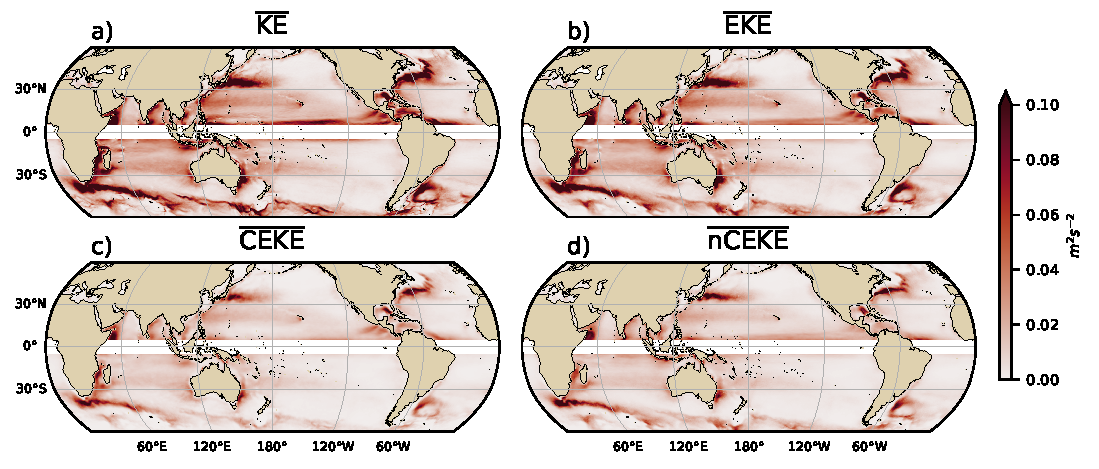
\includegraphics[width=1\textwidth]{figures/mean_ke_maps_satellite.pdf}
	    \caption{Mean surface kinetic energy ($\MKE$), surface eddy kinetic energy ($\MEKE$), surface coherent eddy kinetic energy ($\MCEKE$), and surface non-coherent eddy kinetic energy ($\MnCEKE$) \DIFaddbeginFL \DIFaddFL{averaged }\DIFaddendFL between 1993-2018.}
	    \label{fig:eddy_climatology}
	\end{figure}

	% \textbf{Figure 3}
	% \begin{itemize}
		% \item $\MEKE$ is responsible of almost all the $\MKE$ across the ocean, except for regions with persistent currents over time, such as the mean boundary extension locations, equatorial pacific currents and regions in the Antarctic Circumpolar current, where the EKE explains around 40\% of the $\MKE$
		% \item This estimate is consistent with that of Chelton.
		% \item $\MEKE$ Explains $~80\%$ of $\MKE$, while $\MCEKE$ is $~45\%$ of $\MEKE$ and $\MnCEKE$  is $~60\%$ of $\MEKE$ 
		% \item $\MCEKE$ is large equatorwards from the Kuroshio current and Agulhas current.
		% \item Areas with the largest coherent contribution are located in the South of Australia $\MCEKE$ and South Atlantic
		% \item 
		% \item $\MnCEKE$ has a large amount of energy at high latitudes, this could be a consequence of the satellites not resolving the mesoscale coherent eddies. 
	% 	\item Global averages of the ratios show $\MEKE$ explains around 78\% of the ocean $\MKE$ field, while coherent eddies and non coherent eddy features contain 49\% and 59\% percent. Note this values don't add to 1 as there are cross terms that contain around XX\% of the total energy.
	% \end{itemize}


	\begin{figure}
	    \centering
	    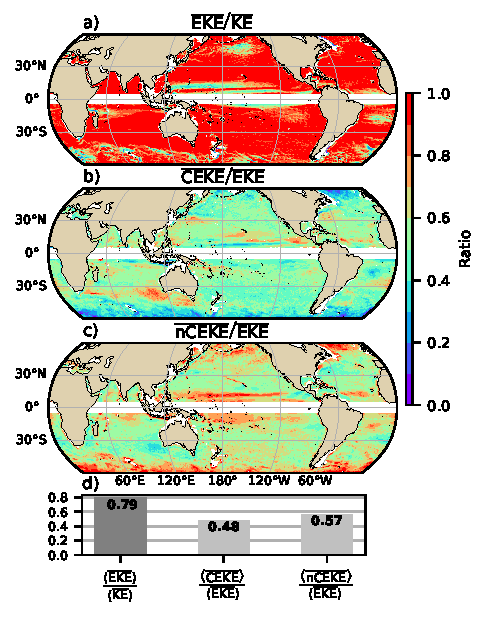
\includegraphics[width=1\textwidth]{figures/eke_ratio_map_easy.pdf}
	    \caption{Ratios of the kinetic energy components. a) Map of the proportion of mean eddy kinetic energy ($\MEKE$) versus mean kinetic energy ($\MKE$);
		b) Map of the percentage of mean coherent eddy kinetic energy ($\MCEKE$) versus mean eddy kinetic energy ($\MEKE$);
		c) Map of the percentage of mean non-coherent eddy kinetic energy ($\MnCEKE$) versus mean eddy kinetic energy ($\MEKE$);
		d) Global time and area averaged (represented by $\left<\,\right>$) percentage of mean eddy kinetic energy ($\left<\MEKE\right>$) versus the global mean kinetic energy ($\left<\MKE\right>$), area averaged percentage of mean coherent eddy kinetic energy ($\left<\MCEKE\right>$) and mean non coherent eddy kinetic energy ($\left<\MnCEKE\right>$) versus global mean eddy kinetic energy ($\left<\MEKE\right>$). Regions where the depth of the ocean is shallower than 1000m are removed from the ratio estimation.
		}
	    \label{fig:eddy_ratio}
	\end{figure}

	Eddy kinetic energy is known to be more than an order of magnitude greater than \DIFaddbegin \DIFadd{kinetic energy of the mean flow (}\DIFaddend $\mKE$\DIFdelbegin \DIFdel{\mbox{%DIFAUXCMD
\citep{Gill_Energy_1974}}\hspace{0pt}%DIFAUXCMD
; }\DIFdelend \DIFaddbegin \DIFadd{; \mbox{%DIFAUXCMD
\citealp{Gill_Energy_1974}}\hspace{0pt}%DIFAUXCMD
); }\DIFaddend this result is clearly shown in Figure \ref{fig:eddy_ratio}a, \DIFdelbegin \DIFdel{where }\DIFdelend \DIFaddbegin \DIFadd{which indicates that }\DIFaddend $\MEKE$ is responsible for almost all the $\MKE$ across the ocean, except for regions with persistent currents over time. 
	Such regions are located in the mean boundary extension locations, the equatorial Pacific currents and regions in the Antarctic Circumpolar Current, where the $\MEKE$ explains around 40\% of the $\MKE$. 
	In a previous study, \citet{Chelton_The_2011} estimated that the $\EKE$ within coherent eddies with lifetimes greater than 4 weeks contain between \DIFdelbegin \DIFdel{40 to 60 percent }\DIFdelend \DIFaddbegin \DIFadd{40-60\% }\DIFaddend of the $\MEKE$. 
	Our method to reconstruct the coherent eddy signature (Figure \ref{fig:eddy_ratio}b) further corroborates that the coherent \DIFaddbegin \DIFadd{eddy }\DIFaddend component ($\left<\MCEKE\right>$) has $\sim$48\% of the $\left<\MKE\right>$ (Figure \ref{fig:eddy_ratio}d). 
	Furthermore, global area averages of the ratios show \DIFaddbegin \DIFadd{that }\DIFaddend $\left<\MEKE\right>$ explains $\sim$78\% of the ocean $\left<\MKE\right>$ field, while non coherent eddy features contain $\sim$57\% percent of the $\left<\MEKE\right>$. 
	Note \DIFaddbegin \DIFadd{that }\DIFaddend the globally averaged coherent and non coherent components do not add to 100\% as the cross terms ($\mathcal{O}_c^2$) are non-zero \DIFdelbegin \DIFdel{, due to }\DIFdelend \DIFaddbegin \DIFadd{and }\DIFaddend coherent eddy reconstruction errors.
	The spatial pattern reveals a dominance of the $\MCEKE$ equatorward from the boundary \DIFdelbegin \DIFdel{extensions and }\DIFdelend \DIFaddbegin \DIFadd{current extensions and in }\DIFaddend areas with large coherent eddy contributions of around 80\% of the region's eddy kinetic energy\DIFdelbegin \DIFdel{can be found }\DIFdelend \DIFaddbegin \DIFadd{, such as }\DIFaddend south of Australia, \DIFaddbegin \DIFadd{in }\DIFaddend the Tehuantepec Gulf, and \DIFaddbegin \DIFadd{in }\DIFaddend the tropical Atlantic. 
	An evident signal is \DIFdelbegin \DIFdel{an }\DIFdelend \DIFaddbegin \DIFadd{a }\DIFaddend reduction of the energy contained by coherent eddies at high latitudes and an increase in the energy explained by non-coherent eddies; this signal could be a consequence of the \DIFdelbegin \DIFdel{incapability }\DIFdelend \DIFaddbegin \DIFadd{inability }\DIFaddend of the 0.25$^\circ$ satellite resolution ($\sim$ 13 km at 60$^\circ$ \DIFaddbegin \DIFadd{latitude}\DIFaddend ) to resolve coherent eddies with scales smaller than $\sim$10 km (first baroclinic Rossby radius at 60$^\circ$; \DIFdelbegin \DIFdel{\mbox{%DIFAUXCMD
\citealt{Chelton_Geographical_1998}}\hspace{0pt}%DIFAUXCMD
}\DIFdelend \DIFaddbegin \DIFadd{\mbox{%DIFAUXCMD
\citealp{Chelton_Geographical_1998}}\hspace{0pt}%DIFAUXCMD
}\DIFaddend ).

	% \subsection{Seasonality}

	% \textbf{Figure 4}
	% \begin{itemize}
		% \item The hemisphere seasonality show the  $\EKE$ and $\CEKE$ peak in summer.
		% \item Response of the $\EKE$ and $\CEKE$ show a seasonal lag of $\sim$6 months to the forcing of the Winds. Make sure to note the maximum over the hemisphere, locally, the winds may peak in different months. 
		% \item The coherent eddy field show a large interannual variability.
		% \item In the Southern Ocean we observe a concentric growth as time passes, which support the increasing trends in the Southern Ocean observed by \citep{Hogg_Recent_2015,Martinez_TKE_2019,Martinez_Kinetic_2021}
		% \item Point that in the northern hemisphere in winter the CEKE appears to be decreasing.
	% \end{itemize}

	Figure \ref{fig:eddy_energy_polar} shows the seasonal cycle of the area weighted $\EKE$ and $\CEKE$ for the Northern Hemisphere ($\left< \EKE\right>_{NH}$ and $\left< \CEKE\right>_{NH}$; 10$^\circ$N - 60$^\circ$N) and Southern Hemisphere ($\left< \EKE\right>_{SH}$  and $\left< \CEKE\right>_{SH}$; 60$^\circ$S - 10$^\circ$S). 
	In both hemispheres, the $\left<\EKE\right>$ and $\left<\CEKE\right>$ peak during summer. In the Northern Hemisphere, the largest $\left<\EKE\right>_{NH}$ and $\left<\CEKE\right>_{NH}$ occurs in July, $\sim$6 months after the maximum winds in January (purple bar and back star in Figure \ref{fig:eddy_energy_polar}c and d). Meanwhile, the Southern Ocean 
	$\left<\EKE\right>_{SH}$ and $\left<\CEKE\right>_{SH}$ seasonal maxima arises during December, $\sim$4 months after the maximum winds in August (purple bar and back star in Figure \ref{fig:eddy_energy_polar}g, and h). This lag between winds and the eddy and coherent eddy energy components is further discussed in \DIFdelbegin \DIFdel{section }\DIFdelend \DIFaddbegin \DIFadd{Section }\DIFaddend \ref{sec:CE_stats}.

	The cyclic plots in Figure \ref{fig:eddy_energy_polar} show the temporal evolution of $\left<\EKE\right>$ and $\left<\CEKE\right>$. 
	Note that high frequency variability can be observed in the $\left<\CEKE\right>$ field with temporal scales of a few months, this \DIFaddbegin \DIFadd{variability }\DIFaddend could be attributed \DIFdelbegin \DIFdel{local }\DIFdelend \DIFaddbegin \DIFadd{to regional }\DIFaddend dynamics averaged over the hemisphere \DIFdelbegin \DIFdel{, }\DIFdelend \DIFaddbegin \DIFadd{(boundary currents, ocean gyres, etc.), }\DIFaddend as well as errors within the coherent eddy reconstruction. 
	% This signature will be further explored in section \ref{sec:CE_regional_stats}.
	Additionally, concentric changes in the cyclic plots highlight long-term changes over the record. For example, the Northern Hemisphere winters \DIFdelbegin \DIFdel{in }\DIFdelend \DIFaddbegin \DIFadd{during }\DIFaddend early years of the record (blue) had a more energetic coherent eddy field, which has transitioned to weaker coherent energy \DIFdelbegin \DIFdel{contents }\DIFdelend \DIFaddbegin \DIFadd{content }\DIFaddend since 2010 (red), in other words, the intensity of the $\left<\CEKE\right>_{NH}$ field has decreased. A larger long-term change can be observed in the Southern Hemisphere, where concentric growth over time in $\left<\EKE\right>_{SH}$ and $\left<\CEKE\right>_{SH}$ support the previously observed strengthening of the eddy field in the Southern Ocean \citep{Hogg_Recent_2015,Martinez_TKE_2019,Martinez_Kinetic_2021}. 

	\begin{figure}
	    \centering
	    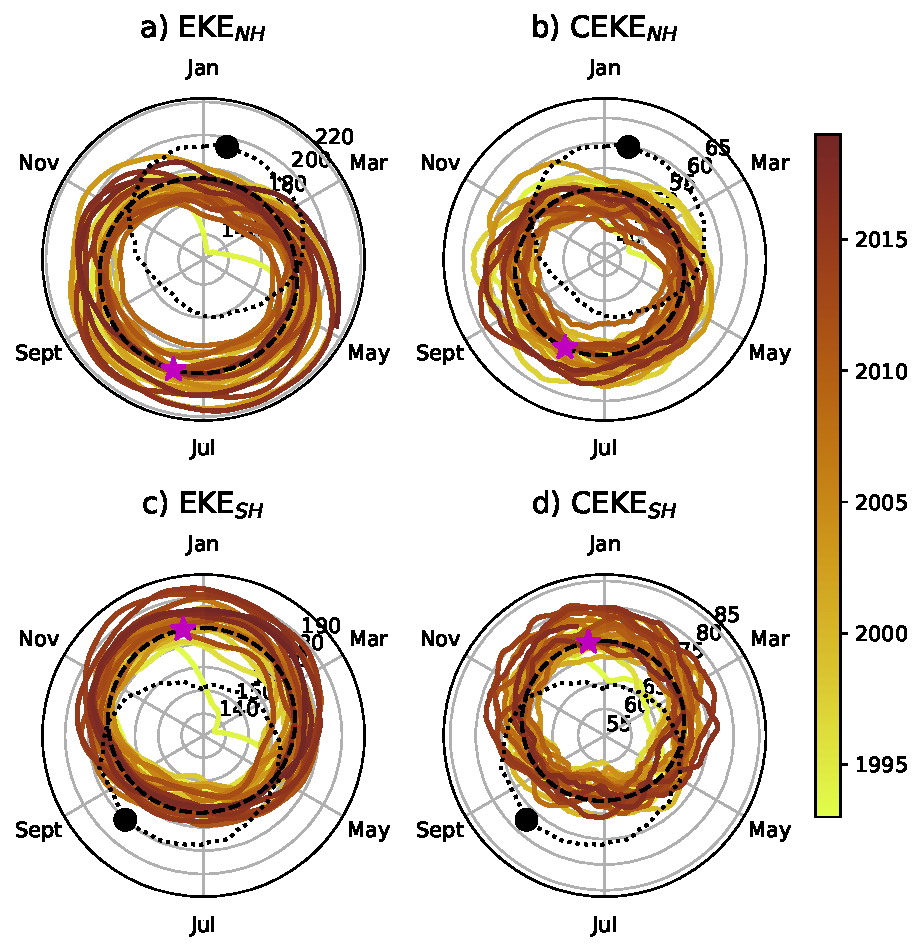
\includegraphics[width=95mm]{figures/All_polar_plots.pdf}
	    \caption{Seasonality of the \DIFdelbeginFL \DIFdelFL{area weighted }\DIFdelendFL \DIFaddbeginFL \DIFaddFL{area-weighted }\DIFaddendFL eddy kinetic energy ($\left<\EKE\right>$) \DIFdelbeginFL \DIFdelFL{, }\DIFdelendFL \DIFaddbeginFL \DIFaddFL{and }\DIFaddendFL coherent eddy kinetic energy ($\left<\CEKE\right>$). 
		Panels a\DIFaddbeginFL \DIFaddFL{) }\DIFaddendFL and b\DIFaddbeginFL \DIFaddFL{) }\DIFaddendFL show the time-series of the Northern Hemisphere, while panels e\DIFaddbeginFL \DIFaddFL{) }\DIFaddendFL and f\DIFaddbeginFL \DIFaddFL{) }\DIFaddendFL correspond to the Southern Hemisphere. Panels c\DIFaddbeginFL \DIFaddFL{) }\DIFaddendFL and d\DIFaddbeginFL \DIFaddFL{) }\DIFaddendFL show the seasonal cycle of the $\left<\EKE\right>_{NH}$ and $\left<\CEKE\right>_{NH}$ in the Northern Hemisphere, and panels g\DIFaddbeginFL \DIFaddFL{) }\DIFaddendFL and h\DIFaddbeginFL \DIFaddFL{) }\DIFaddendFL show the Southern Hemisphere ($\left<\EKE\right>_{SH}$ and $\left<\CEKE\right>_{SH}$).
		Dashed lines correspond to the seasonal cycle of the fields and dotted lines show the seasonal cycle of the wind magnitude smoothed over 120 days (moving average). 
		The black and magenta markers (circle and bar) show the maximum of the seasonal cycle for the kinetic energy components and the wind magnitude, respectively. In \DIFaddbeginFL \DIFaddFL{the }\DIFaddendFL cyclic plots, line colors shows the year.}
	    \label{fig:eddy_energy_polar}
	\end{figure}

	\section{Global Coherent Eddy Statistics}
	\label{sec:CE_stats}

	% \textbf{Figure 5}
	% \begin{itemize}
		% \item A comparison with previous identified numbers show a consistent pattern in the eddy count. The difference in the magnitude could be a consequence of \citet{Chelton_Global_2007} filtering the coherent eddies with lifespans longer than 16 weeks. 
		% \item Both datasets show a large number of eddies in the East North Pacific, East North Atlantic, as well as the East South Pacific, East South Atlantic and East Indian Ocean. 
		% \item While the number of eddies detected in the tropics is quite small.
		% \item Furthermore, there are hotspots of numbers of eddies in other regions of the ocean, such as boundary extensions and the Antarctic Circumpolar Current. 
		% \item An interesting feature shown in both datasets is a predominant patchiness where the count of the eddies is much larger. These puzzling pattern remains unknown. Although it looks like a propagation pattern, it could be that eddies persist for longer in those areas.
		% \item The eddy amplitude as expected is maximum at the boundary extensions and hotspots in the southern ocean.
		% \item Interior of the gyres we can observe that there is and important amplitude of the coherent eddy field. 
		% \item Preferred eddy amplitude sign in boundary extensions; positive amplitude polewards to the boundary extension mean location, and negative amplitude equatorwards. This is consistent with the shed of coherent eddies from the boundary extensions.
		% \item There regions with large $\CEKE$ ratio show also a large coherent eddy amplitude.
		% \item Absolute eddy amplitude has the similar signature as CEKE.
	% \end{itemize}

	Coherent eddy kinetic energy allows us to quantify and study the energy of the eddy field, but the coherent eddy properties computed by automated coherent eddy identification algorithms allow us \DIFaddbegin \DIFadd{to further }\DIFaddend investigate in more detail the contribution and temporal changes of their abundance (\DIFaddbegin \DIFadd{i.e.}\DIFaddend the number of eddies) and their intensity (both their amplitude and diameter). 
	Figure \ref{fig:eddy_stats_climatology} shows gridded climatologies of the number of eddies and the eddy amplitude. 
	\DIFdelbegin \DIFdel{We contrast our M-M }\DIFdelend \DIFaddbegin \DIFadd{In this analysis, we contrast our MM19 }\DIFaddend eddy count with \DIFdelbegin \DIFdel{\mbox{%DIFAUXCMD
\citet{Chelton_Global_2007} }\hspace{0pt}%DIFAUXCMD
(}\DIFdelend \DIFaddbegin \DIFadd{that of CS13 (\mbox{%DIFAUXCMD
\citealp{Chelton_Global_2007}}\hspace{0pt}%DIFAUXCMD
; }\DIFaddend Figure \ref{fig:eddy_stats_climatology}a-b). Although the number of \DIFdelbegin \DIFdel{the }\DIFdelend identified eddies is larger in \DIFdelbegin \DIFdel{M-M}\DIFdelend \DIFaddbegin \DIFadd{MM19}\DIFaddend , possibly due to the lifespan filter implemented by \DIFdelbegin \DIFdel{Chelton}\DIFdelend \DIFaddbegin \DIFadd{CS13}\DIFaddend , both datasets reveal consistent spatial patterns. 
	For example, both datasets show \DIFdelbegin \DIFdel{high }\DIFdelend \DIFaddbegin \DIFadd{an important zonal variation in the }\DIFaddend abundance of eddies\DIFdelbegin \DIFdel{in the }\DIFdelend \DIFaddbegin \DIFadd{, with high numbers of eddies in mid-latitudes and fewer eddies in the tropics and at high-latitudes ($\sim$60$^\circ$). Additionally, there is a tendency at mid-latitudes (30$^\circ$) of higher number of eddies in the eastern side of ocean basins (e.g. }\DIFaddend East North Pacific, East North Atlantic, \DIFdelbegin \DIFdel{as well as the }\DIFdelend East South Pacific, \DIFaddbegin \DIFadd{and }\DIFaddend East South Atlantic\DIFdelbegin \DIFdel{and East Indian Ocean, and small number counts of eddies in the tropics and in high latitudes ($\sim$60$^\circ$). 
	An interesting pattern also }\DIFdelend \DIFaddbegin \DIFadd{). 
	Another interesting pattern }\DIFaddend emerges in both eddy count datasets, where small scale structures \DIFdelbegin \DIFdel{with larger eddy counts are favored across the ocean. 
	In addition, to preferential }\DIFdelend \DIFaddbegin \DIFadd{appear in the eddy count field. 
	These small structures highlight preferred }\DIFaddend coherent eddy paths observable in boundary \DIFdelbegin \DIFdel{extensions and regions in }\DIFdelend \DIFaddbegin \DIFadd{current extensions and over regions of }\DIFaddend the Southern Ocean. 
	These \DIFdelbegin \DIFdel{clusters }\DIFdelend \DIFaddbegin \DIFadd{structures }\DIFaddend and paths of coherent eddies could be associated with topographic features, \DIFdelbegin \DIFdel{however they remain a puzzling }\DIFdelend \DIFaddbegin \DIFadd{with overall }\DIFaddend consistency between the eddy count \DIFdelbegin \DIFdel{pattern using these two }\DIFdelend \DIFaddbegin \DIFadd{patterns using the two different }\DIFaddend eddy identification methods.

	\begin{figure}
	    \centering
	    \includegraphics[width=1\textwidth]{figures/global_stats_V1.pdf}
	    \caption{Averaged coherent eddy statistics. a) Climatology of the number of coherent eddies ($\cEddy_n$) identified by \citet{Chelton_Global_2007};  b) Climatology of the number of coherent eddies ($\cEddy_n$) identified by \citet{Martinez_TKE_2019}; c) Climatology of the mean absolute coherent eddy amplitude ($\cEddy_{amp}$). d) Climatology of the mean coherent eddy amplitude ($\cEddy_{amp}$).}
	    \label{fig:eddy_stats_climatology}
	\end{figure}

	Regions with large counts of eddies have in general small absolute amplitudes (Figure \ref{fig:eddy_stats_climatology} c)\DIFdelbegin \DIFdel{, }\DIFdelend \DIFaddbegin \DIFadd{.
	The }\DIFaddend ocean gyre interiors \DIFdelbegin \DIFdel{follow with }\DIFdelend \DIFaddbegin \DIFadd{have }\DIFaddend a larger absolute amplitude and finally regions such as the boundary \DIFdelbegin \DIFdel{extensions and }\DIFdelend \DIFaddbegin \DIFadd{current extensions and the }\DIFaddend Antarctic Circumpolar Current have the largest coherent eddy absolute amplitudes\DIFdelbegin \DIFdel{as shown }\DIFdelend \DIFaddbegin \DIFadd{, as shown also }\DIFaddend by \citet{Chelton_The_2011}.
	Eddy amplitude highlights regions dominated by a given coherent eddy polarity, for example, boundary extensions have a preferred sign (Figure \ref{fig:eddy_stats_climatology} d); \DIFaddbegin \DIFadd{namely, }\DIFaddend positive amplitude polewards of the boundary \DIFaddbegin \DIFadd{current }\DIFaddend extension mean location, and negative amplitude equatorwards. 
	This sign preference is consistent with the preferential way \DIFaddbegin \DIFadd{that }\DIFaddend coherent eddies are shed from boundary \DIFdelbegin \DIFdel{extensions; }\DIFdelend \DIFaddbegin \DIFadd{current extensions; with }\DIFaddend warm core eddies (positive)  polewards of the boundary current extension, and equatorward for cold core eddies (negative) \DIFdelbegin \DIFdel{\mbox{%DIFAUXCMD
\citep{Kang_eddy_characteristics_2013,Chelton_The_2011,Chelton_Global_2007}}\hspace{0pt}%DIFAUXCMD
}\DIFdelend \DIFaddbegin \DIFadd{\mbox{%DIFAUXCMD
\citep{Chelton_Global_2007,Chelton_The_2011,Kang_eddy_characteristics_2013}}\hspace{0pt}%DIFAUXCMD
}\DIFaddend . 
	These global statistics reveal the absolute coherent eddy amplitude \DIFdelbegin \DIFdel{is a proxy of }\DIFdelend \DIFaddbegin \DIFadd{as a proxy for }\DIFaddend the $\CEKE$ with similar spatial patterns (Figure \ref{fig:eddy_climatology} \& Figure \ref{fig:eddy_stats_climatology}c) and showcases that regions where $\MCEKE$ has a large proportion of $\MEKE$ (Figure \ref{fig:eddy_ratio}), the absolute coherent eddy amplitude is also large.

	% \subsection{Seasonality}
	% \label{subsec:CE_season}

	% \textbf{Figure 6}
	% \begin{itemize}
		% \item Seasonality of the number of eddies in the Northern Hemisphere peaks on May, while the Southern Hemisphere peaks on October. 
		% \item The seasonality of the amplitude of the eddies is consistent with those of the Coherent eddy kinetic energy. 
		% \item Interestingly, there is a 3 month lag to between the winds and the seasonality of the number of eddies, while the eddy amplitude responds approximately 6 months after the maximum winds. 
		% \item Note that both coherent eddy amplitudes seem to peak around the same time. 
		% \item If we look closely, the growing-shrinking concentric circles correspond to an increasing-decreasing trend. These are particularly obvious as a decrease in the eddy number in the Southern Hemisphere, and a increase in the eddy amplitude. 
	% \end{itemize}


	To further understand the seasonal cycle of $\left<\CEKE\right>$, we compute the climatology of coherent eddy properties in each hemisphere (Figure \ref{fig:eddy_stats}). 
	The seasonality of the number of eddies in the Northern Hemisphere peaks \DIFdelbegin \DIFdel{on }\DIFdelend \DIFaddbegin \DIFadd{in }\DIFaddend April (Figure \ref{fig:eddy_stats}\DIFdelbegin \DIFdel{~}\DIFdelend a, c), while the Southern Hemisphere maximum number of eddies occurs during October (Figure \ref{fig:eddy_stats}\DIFdelbegin \DIFdel{~}\DIFdelend e, g). 
	Meanwhile, the seasonality of the \DIFdelbegin \DIFdel{polarity independent }\DIFdelend eddy amplitude ($\left<|\cEddy_{amp}|\right>$) peaks in August and January for the Northern and Southern Hemispheres respectively (Figure \ref{fig:eddy_stats}\DIFdelbegin \DIFdel{~}\DIFdelend b, d, f, and h). 
	As expected, the seasonality of $\left<|\cEddy_{amp}|\right>$\DIFdelbegin \DIFdel{xw, or }\DIFdelend \DIFaddbegin \DIFadd{, }\DIFaddend equivalent to the intensity of the coherent eddies, is consistent with the seasonal cycle of $\left<\CEKE\right>$.
\DIFdelbegin \DIFdel{Furthermore, }\DIFdelend \DIFaddbegin 

	\DIFadd{A key feature of Figure \ref{fig:eddy_stats} is }\DIFaddend a distinct lag of $\sim$3 months \DIFdelbegin \DIFdel{is observed }\DIFdelend between the winds and eddy count, while the eddy amplitude maximum occurs $\sim$6 months after the seasonal maxima in winds. 
	We \DIFdelbegin \DIFdel{observe }\DIFdelend \DIFaddbegin \DIFadd{suggest that }\DIFaddend the eddy number increases earlier in the year and\DIFaddbegin \DIFadd{, }\DIFaddend through eddy-eddy interactions (merging of coherent eddies)\DIFaddbegin \DIFadd{, }\DIFaddend the amplitude of the coherent eddy increases $\sim$3 months after. This seasonal lag and summer maxima is consistent with \DIFdelbegin \DIFdel{Figure \ref{fig:eddy_stats_climatology}, furthermore, previous studies }\DIFdelend \DIFaddbegin \DIFadd{previous studies which }\DIFaddend suggest that a time-lag of the inverse cascade \citep{Sasaki_seasonal_2014, Qiu_seasonal_2014} is responsible \DIFdelbegin \DIFdel{of }\DIFdelend \DIFaddbegin \DIFadd{for }\DIFaddend the $\EKE$ seasonal cycle, where winter has the highest energy at the smallest scales (non-resolvable with satellite observations), spring and autumn have the highest and lowest energy \DIFdelbegin \DIFdel{in }\DIFdelend \DIFaddbegin \DIFadd{at }\DIFaddend scales of 50-100 km, and summertime has the highest energy at the largest scales ($>$ 100 km; \DIFdelbegin \DIFdel{\mbox{%DIFAUXCMD
\citealt{Uchida_Seasonality_2017}}\hspace{0pt}%DIFAUXCMD
}\DIFdelend \DIFaddbegin \DIFadd{\mbox{%DIFAUXCMD
\citealp{Uchida_Seasonality_2017}}\hspace{0pt}%DIFAUXCMD
}\DIFaddend ). 
	Thus, the maximum of $\left<\EKE\right>$, $\left<\CEKE\right>$, and $\left<|\cEddy_{amp}|\right>$ located during summertime \DIFdelbegin \DIFdel{suggest }\DIFdelend \DIFaddbegin \DIFadd{suggests }\DIFaddend that the seasonality of eddies and coherent eddies could be dominated by scales larger than 100 km.
\DIFaddbegin 

	\DIFaddend This result can be further explored by looking at the seasonal evolution of the eddy diameter ($\cEddy_d$). 
	Note that 90\% of identified coherent eddies have diameters between 50 to 220 km (Figure \ref{fig:eddy_diameter}\DIFdelbegin \DIFdel{~}\DIFdelend a). We \DIFdelbegin \DIFdel{divided }\DIFdelend \DIFaddbegin \DIFadd{partition }\DIFaddend eddies into large-scale coherent eddies (diameter $>$ 120 km) and  small-scale coherent eddies (diameter $<$ 120 km; Figure \ref{fig:eddy_diameter}a). 
	In the Northern Hemisphere, \DIFdelbegin \DIFdel{small }\DIFdelend \DIFaddbegin \DIFadd{small-scale }\DIFaddend eddies have a seasonal peak in diameter during May, while \DIFdelbegin \DIFdel{large }\DIFdelend \DIFaddbegin \DIFadd{large-scale }\DIFaddend eddies have the greatest diameter in September (Figure \ref{fig:eddy_diameter}\DIFdelbegin \DIFdel{~}\DIFdelend b).
	Meanwhile, in the Southern Hemisphere, the small-scale coherent eddies \DIFdelbegin \DIFdel{have the }\DIFdelend \DIFaddbegin \DIFadd{exhibit }\DIFaddend maximum diameter in December, while \DIFaddbegin \DIFadd{the diameter of }\DIFaddend large-scale coherent eddies \DIFdelbegin \DIFdel{peak }\DIFdelend \DIFaddbegin \DIFadd{peaks }\DIFaddend in February (Figure \ref{fig:eddy_diameter}~c). 
	This result suggests that wind driven baroclinic instabilities generate small coherent eddies early in the season, which then merge and grow to become larger in diameter and amplitude, and thus, more energetic. 
	This process is \DIFaddbegin \DIFadd{likely }\DIFaddend associated with the inverse energy cascade, and \DIFdelbegin \DIFdel{suggest }\DIFdelend \DIFaddbegin \DIFadd{suggests }\DIFaddend that this mechanism not only drives \DIFdelbegin \DIFdel{the }\DIFdelend $\EKE$ seasonality, but also may be responsible \DIFdelbegin \DIFdel{of }\DIFdelend \DIFaddbegin \DIFadd{for }\DIFaddend the seasonal cycle of coherent eddies. 

	%Furthermore, by analogy we extend the argument that a long-term decrease in the number of coherent eddies and increase in coherent eddy amplitude could be a consequence of a long-term increase in the energy cascade, where interactions between eddies may become more frequent and result in stronger coherent eddies. 
	%This hypothesis may also occur in conjunction with other processes, such as baroclinic and barotropic instabilities generating stronger eddies. 

	\begin{figure}
	    \centering
	    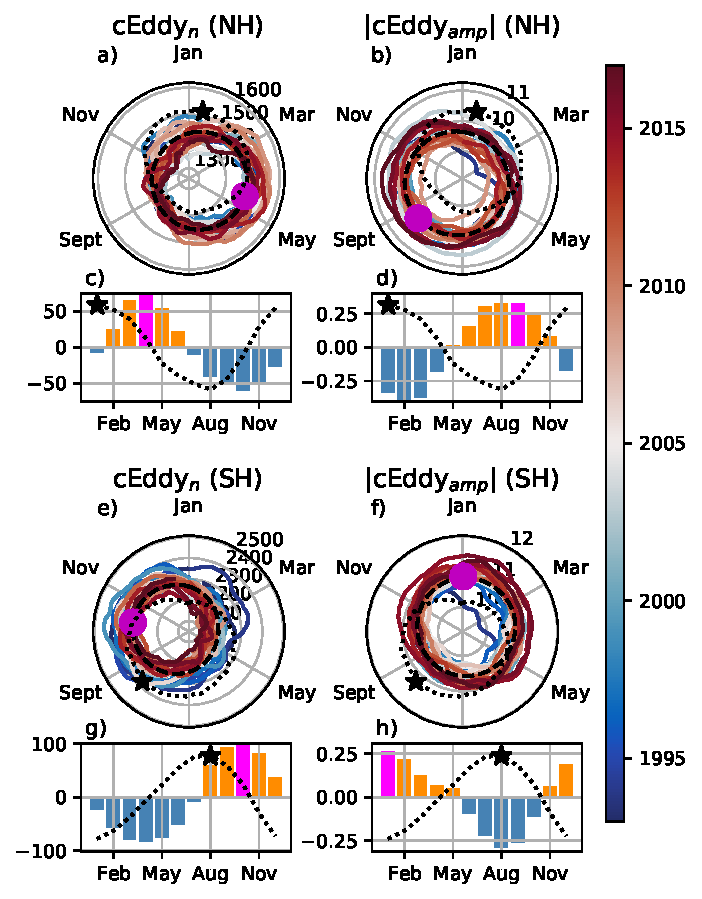
\includegraphics[width=95mm]{figures/All_polar_plots_eddy_stats_polarity_V3.pdf}
	    \caption{
		Seasonality of the count of number of eddies ($\cEddy
		_n$) and \DIFdelbeginFL \DIFdelFL{area weighted }\DIFdelendFL \DIFaddbeginFL \DIFaddFL{the area-weighted }\DIFaddendFL polarity independent coherent eddy amplitude ($\left<\cEddy_{amp}\right>$); Panels a and b show the time-series of the Northern Hemisphere, while panels e and f correspond to the Southern Hemisphere. Panels c and d show the seasonal cycle of the $\cEddy_n$ and $\left<|\cEddy|_{amp}\right>_{NH}$ in the Northern Hemisphere, and panels g and h show the Southern Hemisphere \DIFdelbeginFL \DIFdelFL{(}\DIFdelendFL $\cEddy_n$ and $\left<|\cEddy|_{amp}\right>_{SH}$\DIFdelbeginFL \DIFdelFL{)}\DIFdelendFL .
		Dashed lines correspond to the seasonal cycle of the fields and dotted lines show the seasonal cycle of the wind magnitude\DIFaddbeginFL \DIFaddFL{, }\DIFaddendFL smoothed over 120 days (moving average). 
		The black and magenta markers (circle and bar) \DIFdelbeginFL \DIFdelFL{show }\DIFdelendFL \DIFaddbeginFL \DIFaddFL{indicate }\DIFaddendFL the maximum of the seasonal cycle for the eddy property\DIFaddbeginFL \DIFaddFL{, }\DIFaddendFL and the wind magnitude, respectively. In \DIFaddbeginFL \DIFaddFL{the }\DIFaddendFL cyclic plots, line colors \DIFdelbeginFL \DIFdelFL{shows }\DIFdelendFL \DIFaddbeginFL \DIFaddFL{show }\DIFaddendFL the year \DIFaddbeginFL \DIFaddFL{from 1993-2019}\DIFaddendFL .}
	    \label{fig:eddy_stats}
	\end{figure}

	\begin{figure}
	    \centering
	    \DIFdelbeginFL %DIFDELCMD < 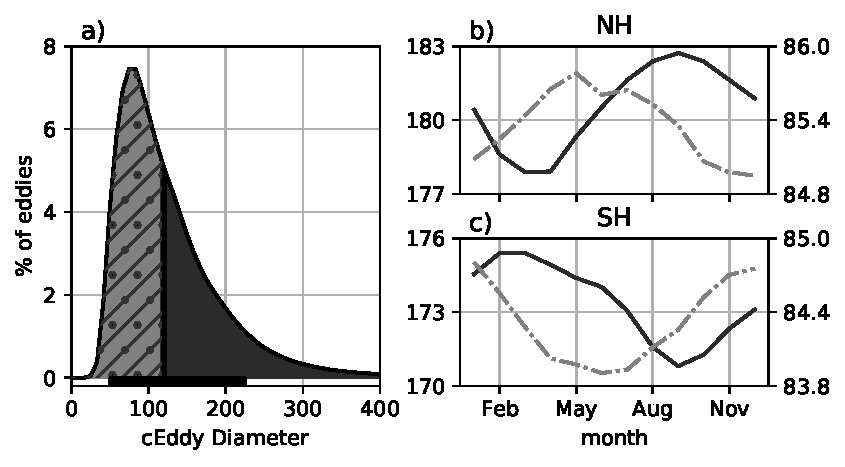
\includegraphics[width=95mm]{figures/eddy_diameter_seasonal.pdf}
%DIFDELCMD < 	    %%%
\DIFdelendFL \DIFaddbeginFL 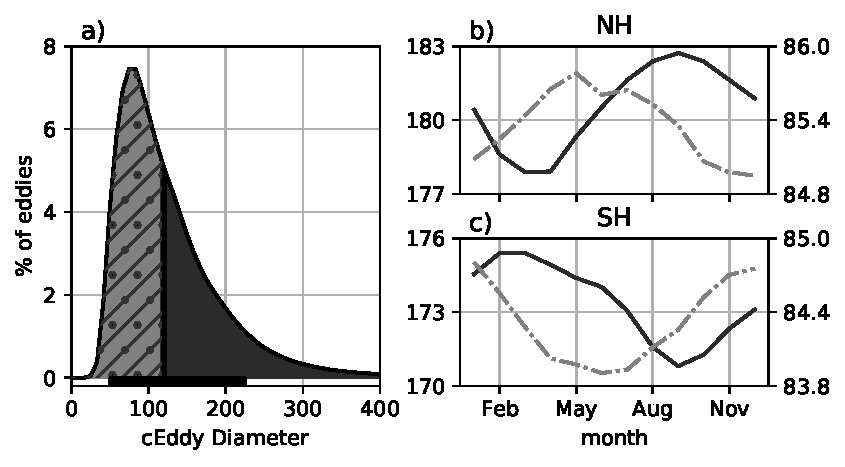
\includegraphics[width=1\textwidth]{figures/eddy_diameter_seasonal.pdf}
	    \DIFaddendFL \caption{Distribution of the identified eddy diameter ($\cEddy_d$; km) and hemispherical seasonality of the coherent eddy diameter. a) Distribution in percentage of identified eddy amplitude, solid bar \DIFdelbeginFL \DIFdelFL{bellow }\DIFdelendFL \DIFaddbeginFL \DIFaddFL{below }\DIFaddendFL distribution represents 90\% of the identified eddies. Seasonal cycle of the eddy diameter for the b) Northern Hemisphere and c) Southern Hemisphere. Dark solid line and area corresponds to coherent eddies with diameters larger than 120 km, while light gray dash-dotted line and area shows coherent eddies with diameters smaller than 120 km.}
	    \label{fig:eddy_diameter}
	\end{figure}

	Long-term changes can be observed in Figure \ref{fig:eddy_stats}a,b, e, and f where \DIFdelbegin \DIFdel{growing-shrinking }\DIFdelend \DIFaddbegin \DIFadd{growing/shrinking }\DIFaddend concentric circles over time denote an \DIFdelbegin \DIFdel{increase-decrease }\DIFdelend \DIFaddbegin \DIFadd{increase/decrease }\DIFaddend trend of the field. 
	This trend is particularly evident in the Southern Hemisphere, where the number of eddies has decreased, \DIFaddbegin \DIFadd{while }\DIFaddend the eddy amplitude has increased. 
	This result is consistent with the observed trends in $\EKE$ and mesoscale $\EKE$ in the Southern Ocean \DIFdelbegin \DIFdel{\mbox{%DIFAUXCMD
\citep{Hogg_Recent_2015,Martinez_TKE_2019}}\hspace{0pt}%DIFAUXCMD
}\DIFdelend \DIFaddbegin \DIFadd{\mbox{%DIFAUXCMD
\citep{Hogg_Recent_2015, Martinez_TKE_2019}}\hspace{0pt}%DIFAUXCMD
}\DIFaddend . The coherent eddy amplitude from positive coherent eddies and negative coherent eddies show similar seasonal cycles to the absolute eddy amplitude. The Northern Hemisphere decrease in absolute eddy amplitude is driven by a decrease of the amplitude of negative coherent eddies in the Northern Hemisphere. Meanwhile in the Southern Ocean, the increase in absolute eddy amplitude is corroborated by \DIFdelbegin \DIFdel{an }\DIFdelend \DIFaddbegin \DIFadd{a }\DIFaddend strengthening of both coherent eddy polarities since the early 90s.

	% Should I add a seasonal cycle of the eddy radius? eddy area?, I've plotted it follows closely the eddy amplitude, which is expected, but as I just argued, the mean seasonal cycle shows on average a peak in summertime with diameters of 90 km, in fact, if I mask the radius with eddies larger than 90km, the seasonal cycle peaks in October, while eddies smaller than 90km peak on May. 

	% \begin{figure}
	%     \centering
	%     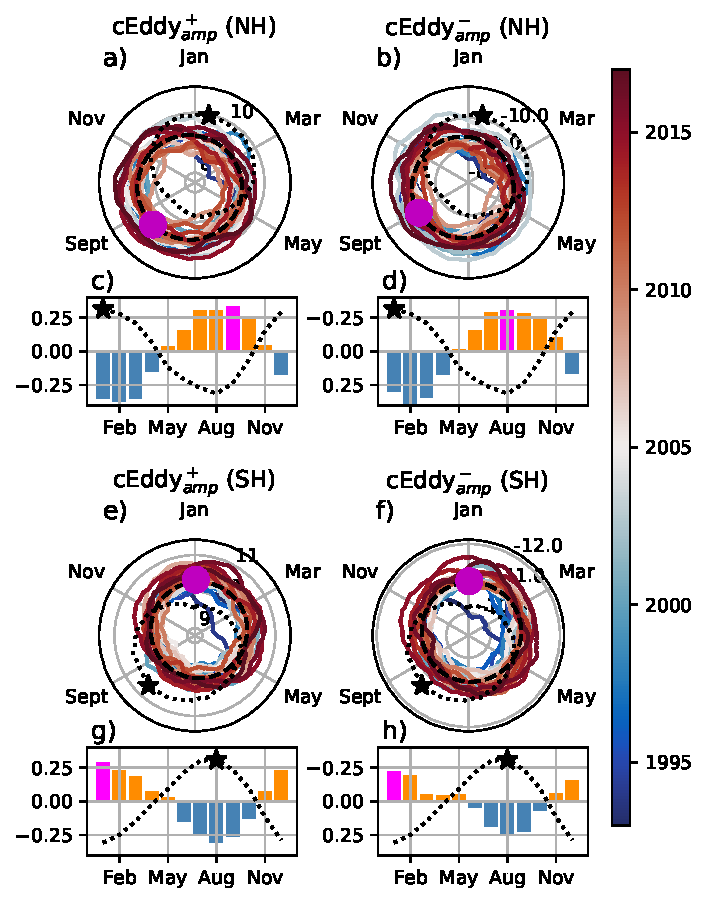
\includegraphics[width=95mm]{figures/All_polar_plots_eddy_stats_polarity_V4.pdf}
	%     \caption{Hemispherical seasonality of the coherent eddy statistics;
	% 	a,e) seasonal cycle of the number of coherent eddies ($\cEddy_n$); b,f) time-series of the mean coherent eddy amplitude ($\cEddy_{amp}$); c,g) seasonal climatology of the warm core coherent eddies amplitude (positive $\cEddy_{amp}$); d,h) seasonal climatology of the cold core coherent eddies amplitude (negative $\cEddy_{amp}$). Panels a, b, c, and d correspond to the Northern Hemisphere, while panels e, f, g, and h correspond to the Southern Hemisphere. Dashed lines correspond to the seasonal cycle of the fields and dotted lines show the seasonal cycle of the wind magnitude smoothed over 120 days (moving average). The green and magenta stars show the maximum of the seasonal cycle for each field and the wind magnitude, respectively. The line colors show the year.}
	%     \label{fig:eddy_stats_polar}
	% \end{figure}

	\section{Trends}
	\label{sec:CE_trends}	

	% \textbf{Figure 13}
	% \begin{itemize}
		% \item The number and amplitude of coherent eddies from two eddy tracking algorithms show consistent trend patterns. 
		% \item In particularly, we observe a decrease in the number of eddies in the southern ocean, as well as sectors in the North Atlantic and North Pacific. 
		% \item Meanwhile the amplitude seems to be increasing in those same regions. 
		% \item Some of these regions have undergone a readjustment to stronger winds, thus the observed trends in the eddy amplitude suggests an intensification of the coherent eddy field to an increase in the forcing.
		% \item This increase is consistent with \citet{Martinez_Kinetic_2021}
	% \end{itemize}

	The results presented in Figures \ref{fig:eddy_energy_polar} and \ref{fig:eddy_stats} suggest a long-term readjustment of the coherent eddy field. 
	The long-term trends of the number of coherent eddies, absolute coherent eddy amplitude, and coherent eddy amplitude polarities are \DIFaddbegin \DIFadd{further }\DIFaddend explored in Figure \ref{fig:eddy_stats_trends} \DIFdelbegin \DIFdel{. 
	Chelton's and M-M }\DIFdelend \DIFaddbegin \DIFadd{contrasting the MM19 and CS13 methods. 
	MM19 and CS13 }\DIFaddend datasets show consistent spatial patterns in the trends and significance of the number of coherent eddies and the absolute coherent eddy amplitude. 
	Several regions in the ocean, such as the Southern Ocean, North Atlantic and North Pacific, show a decrease in the number of eddies. Those same regions also have a clear increase in the absolute coherent eddy amplitude. 
	%This collocation of decrease in number and increase in eddy amplitude provides more evidence of a possible intensification of the coherent eddy field though eddy-eddy interactions. 
	These trends are similar to those observed in mesoscale eddy kinetic energy \citep{Martinez_Kinetic_2021} and provide additional evidence of a readjustment of the mesoscale eddy field over the last 3 decades. 

	\DIFdelbegin \DIFdel{\textcolor{purple}{\textbf{@Matt:}\textit{What do you think? Is it important to highlight the trends we observe are different to sea level rise? Or is the next paragraph irrelevant?}}
}%DIFDELCMD < 

%DIFDELCMD < 	%%%
\DIFdelend The observed trends of $\cEddy_{|amp|}$ in several oceanic regions have the same scale as sea level rise ($\sim$3cm per decade)\DIFdelbegin \DIFdel{by }\DIFdelend \DIFaddbegin \DIFadd{. By }\DIFaddend analyzing the positive and negative coherent eddy amplitude\DIFdelbegin \DIFdel{we can discard }\DIFdelend \DIFaddbegin \DIFadd{, we filter out }\DIFaddend the observed trends \DIFdelbegin \DIFdel{correspond to an }\DIFdelend \DIFaddbegin \DIFadd{that come from a net }\DIFaddend increase in sea level. 
	In fact, each coherent eddy polarity has intensified in the Southern Ocean and North East Pacific and Atlantic. 
	In other words, the amplitude of each polarity has increased over time, \DIFaddbegin \DIFadd{and }\DIFaddend thus this strengthening is an intrinsic response of the coherent eddy field. Note that the negative coherent eddy amplitude dominates the global $|\cEddy_{amp}|$ trends (Figure \ref{fig:eddy_stats_trends}e, f). However, different trend \DIFdelbegin \DIFdel{pattern }\DIFdelend \DIFaddbegin \DIFadd{patterns }\DIFaddend can be observed in both positive and negative coherent eddy amplitudes in the \DIFdelbegin \DIFdel{north Atlantic and north }\DIFdelend \DIFaddbegin \DIFadd{North Atlantic and North }\DIFaddend Pacific, where the negative coherent eddy amplitude in the  Western Boundary Currents appears to decrease.

	\begin{figure}
	    \centering
	    \DIFdelbeginFL %DIFDELCMD < 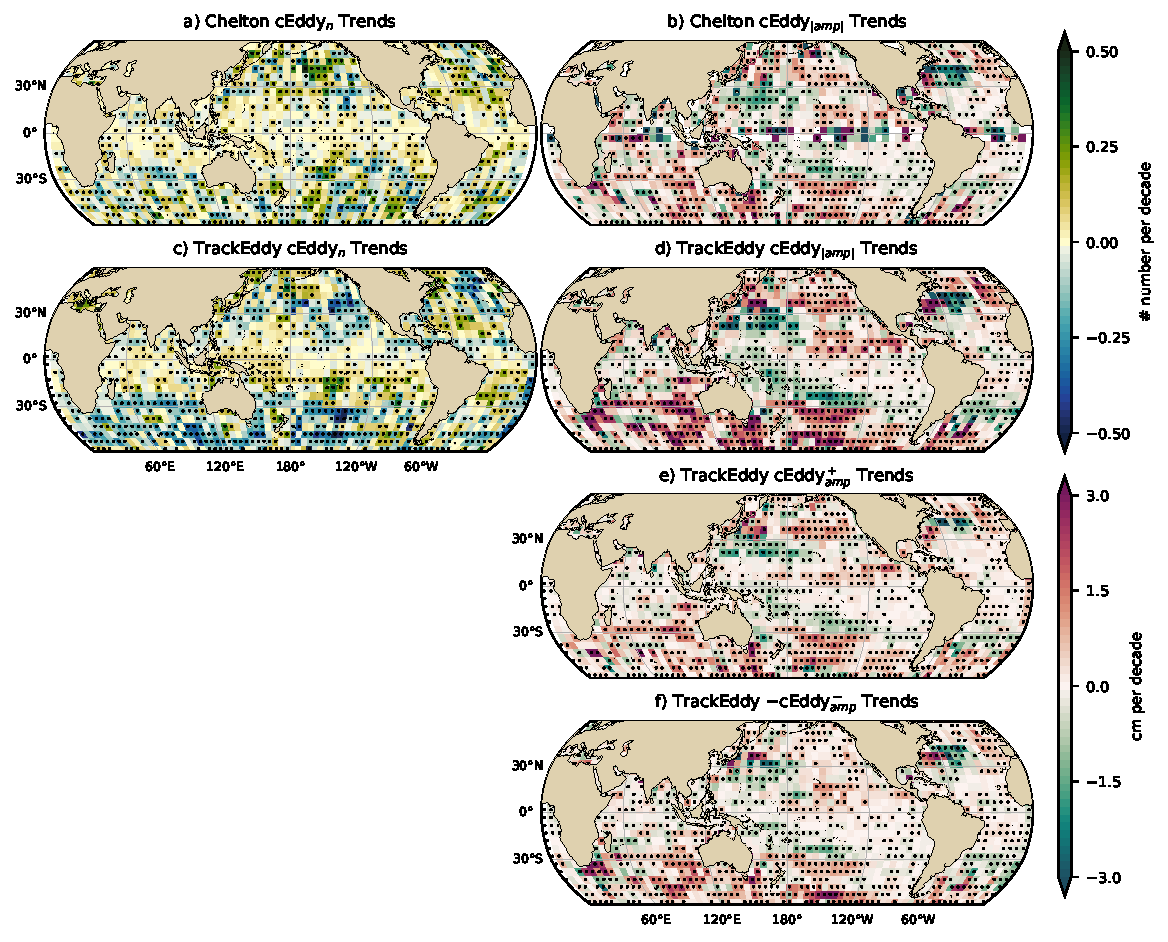
\includegraphics[width=1\textwidth]{figures/all_trackeddy_trends_all.pdf}
%DIFDELCMD < 	    %%%
\DIFdelendFL \DIFaddbeginFL 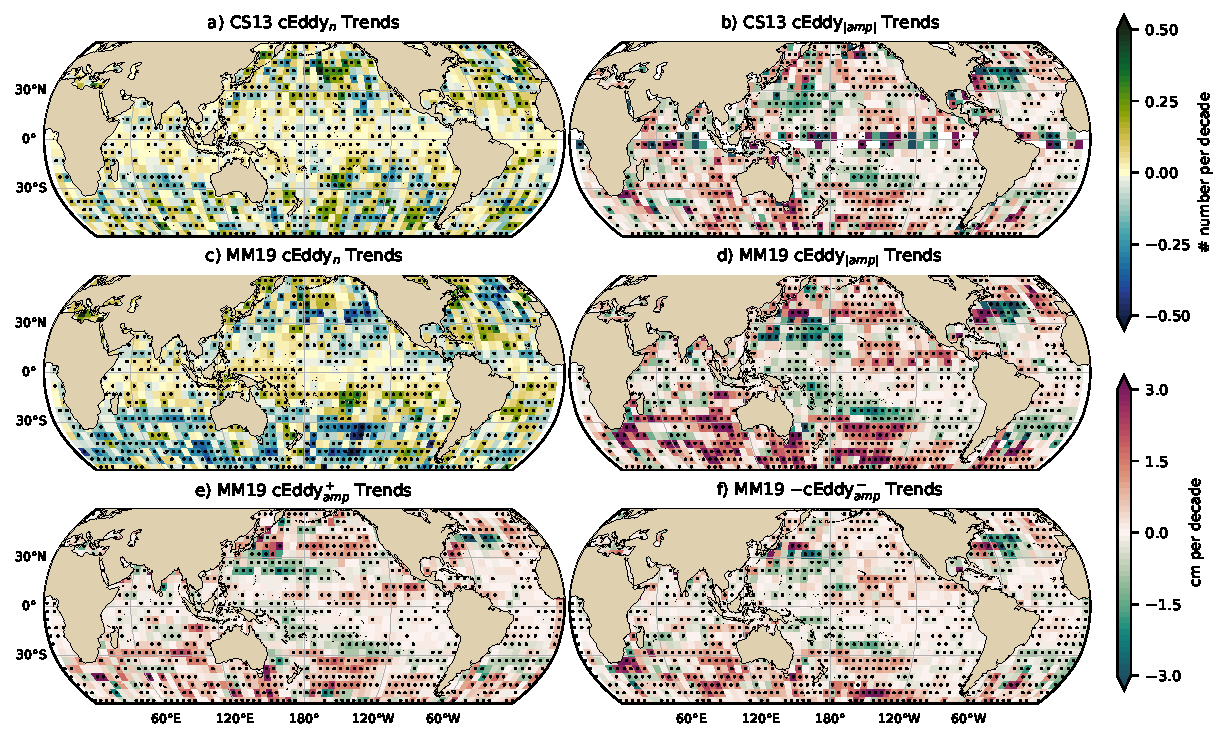
\includegraphics[width=1\textwidth]{figures/all_trackeddy_trends_all_regular.pdf}
	    \DIFaddendFL \caption{Trends of coherent eddy statistics. a) and b) Trends of the number of identified coherent eddies from satellite observations identified using \DIFaddbeginFL \DIFaddFL{the }\DIFaddendFL TrackEddy \DIFaddbeginFL \DIFaddFL{scheme of MM19}\DIFaddendFL , and those reported in \DIFdelbeginFL \DIFdelFL{Chelton}\DIFdelendFL \DIFaddbeginFL \DIFaddFL{CS13}\DIFaddendFL 's dataset. c) and d) Trends of the absolute value of identified coherent \DIFdelbeginFL \DIFdelFL{eddies }\DIFdelendFL \DIFaddbeginFL \DIFaddFL{eddy }\DIFaddendFL amplitude ($\cEddy_{|amp|}$) from satellite observations identified using TrackEddy \DIFaddbeginFL \DIFaddFL{(after MM19)}\DIFaddendFL , and those reported \DIFdelbeginFL \DIFdelFL{in Chelton's dataset}\DIFdelendFL \DIFaddbeginFL \DIFaddFL{by CS13}\DIFaddendFL . e) and f) Trends of \DIFaddbeginFL \DIFaddFL{the }\DIFaddendFL eddy amplitude polarity using TrackEddy ($\cEddy_{amp}^+$ and $\cEddy_{amp}^-$). Gray stippling shows regions that are statistically significant above the 95\% confidence level.}
	    \label{fig:eddy_stats_trends}
	\end{figure}


	% \begin{figure}
	%     \centering
	%     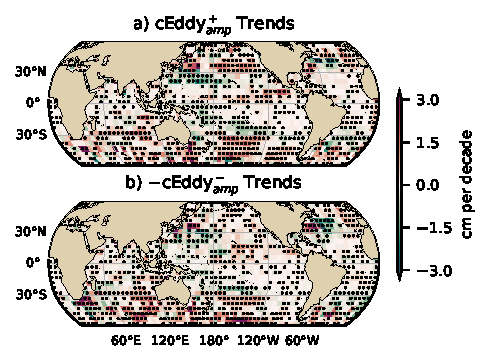
\includegraphics[width=95mm]{figures/all_trackeddy_polarity_amp_trends.pdf}
	%     \caption{Trends of coherent eddy statistics. a) and b) Trends of the number of identified coherent eddies from satellite observations identified using TrackEddy, and those reported in Chelton's dataset. c) and e) Trends of the mean absolute value of identified coherent eddies amplitude from satellite observations identified using TrackEddy, and those reported in Chelton's dataset. Gray stippling shows regions that are statistically significant above the 95\% confidence level.
	% 	}
	%     \label{fig:eddy_stats_amp_trends}
	% \end{figure}

	% \textbf{I would like to merge figure 10 into figure 9, however I'm not sure what may be the best layout. Perhaps remove Chelton's and only mention the similarities or add another column.}

	\section{Regional Climatology}
	\label{sec:CE_regional_stats}

	For regions with relatively large proportions of $\CEKE$ located at \DIFdelbegin \DIFdel{boundary extensions and eastern }\DIFdelend \DIFaddbegin \DIFadd{WBCe and eastern boundary }\DIFaddend currents, we investigate the seasonal and long-term variability of the coherent eddy properties. \DIFdelbegin %DIFDELCMD < 

%DIFDELCMD < 	%%%
%DIF <  \subsection{Boundary Currents}
	%DIFDELCMD < 

%DIFDELCMD < 	%%%
\DIFdelend The most energetic \DIFdelbegin \DIFdel{western boundary extensions include ; }\DIFdelend \DIFaddbegin \DIFadd{WBCe include }\DIFaddend the Gulf Stream, the Kuroshio Current, and the Agulhas Current (Figures \ref{fig:Gulf_Stream}, \ref{fig:Kuroshio}, and \ref{fig:Agulhas}). 
	Coherent eddy generation in boundary \DIFaddbegin \DIFadd{current }\DIFaddend extensions occurs through baroclinic and barotropic instabilities of the mean current, thus all these regions share similar generation dynamics. 
	In all these regions without exception; (i) $\CEKE$ contains \DIFdelbegin \DIFdel{up to 80}\DIFdelend \DIFaddbegin \DIFadd{50-80}\DIFaddend \% of the $\EKE$ in regions \DIFdelbegin \DIFdel{equatorwards }\DIFdelend \DIFaddbegin \DIFadd{equatorward }\DIFaddend from the mean \DIFdelbegin \DIFdel{western boundary extension location}\DIFdelend \DIFaddbegin \DIFadd{WBCe}\DIFaddend , (ii) the number of eddies is consistently \DIFdelbegin \DIFdel{minimal numbers of eddies }\DIFdelend \DIFaddbegin \DIFadd{small }\DIFaddend over the mean \DIFdelbegin \DIFdel{western boundary extension location}\DIFdelend \DIFaddbegin \DIFadd{WBCe}\DIFaddend , and (iii) the eddy amplitude is larger \DIFdelbegin \DIFdel{polewards of the mean western boundary extension location}\DIFdelend \DIFaddbegin \DIFadd{over the mean WBCe}\DIFaddend . 

	In the Gulf Stream, the energy ratio between $\CEKE$ and $\EKE$ is $\sim$56\% (Figure \ref{fig:Gulf_Stream}). 
	The highest energy \DIFdelbegin \DIFdel{content }\DIFdelend \DIFaddbegin \DIFadd{ratio }\DIFaddend occurs in regions with numerous eddies, \DIFdelbegin \DIFdel{and }\DIFdelend collocated with regions where the largest $|\cEddy_{amp}|$ gradients \DIFdelbegin \DIFdel{occurs}\DIFdelend \DIFaddbegin \DIFadd{occur}\DIFaddend . 
	The time series of $\cEddy_{n}$ and $\left<|\cEddy_{amp}|\right>$ are anti-correlated (-0.52), and they display \DIFdelbegin \DIFdel{inter-annual }\DIFdelend \DIFaddbegin \DIFadd{interannual }\DIFaddend and seasonal variability. 
	Although \citet{Chaudhuri_Oscillation_2009} observed \DIFaddbegin \DIFadd{that }\DIFaddend a positive phase of \DIFaddbegin \DIFadd{the }\DIFaddend North Atlantic Oscillation (NAO) \DIFdelbegin \DIFdel{exhibit }\DIFdelend \DIFaddbegin \DIFadd{exhibits }\DIFaddend higher $\EKE$, due to an increase in baroclinic \DIFdelbegin \DIFdel{instabilities}\DIFdelend \DIFaddbegin \DIFadd{instability}\DIFaddend , thus suggesting more coherent eddies, we do not find a correlation between the $\cEddy_{n}$ or the $\left<|\cEddy_{amp}|\right>$ in the Gulf Stream and the NAO index. 
	Similar to the signal observed in the \DIFdelbegin \DIFdel{hemispherical }\DIFdelend \DIFaddbegin \DIFadd{hemispheric }\DIFaddend analysis, the eddy count seasonal cycle follows the wind maximum \DIFdelbegin \DIFdel{after }\DIFdelend \DIFaddbegin \DIFadd{lagging by }\DIFaddend $\sim$3 months, while the amplitude of the coherent eddies lags by $\sim$ 6 months. 

	\begin{figure}
	    \centering
	    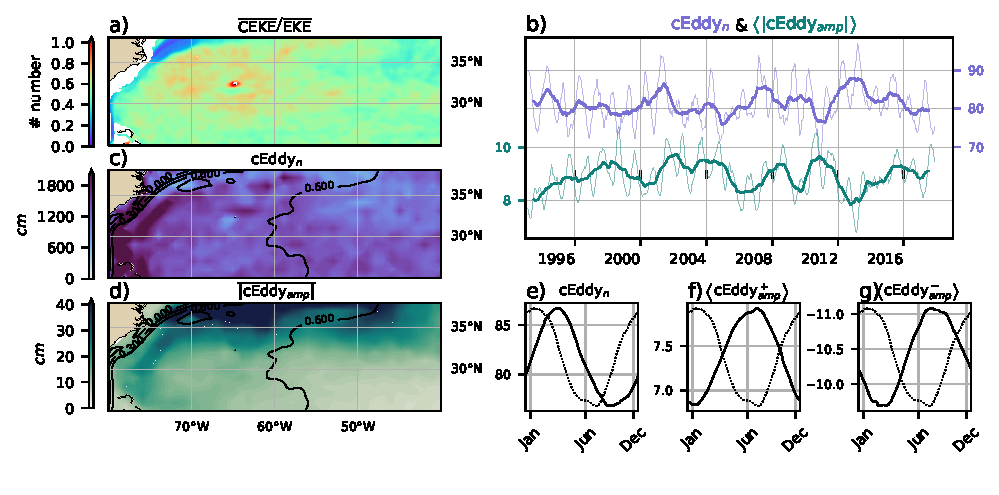
\includegraphics[width=1\textwidth]{figures/regional_ratios_and_stats_V3_5.pdf}
	    \caption{Climatology of the eddy field and coherent eddy field \DIFdelbeginFL \DIFdelFL{at }\DIFdelendFL \DIFaddbeginFL \DIFaddFL{in }\DIFaddendFL the Gulf Stream. a) Ratio of mean coherent eddy kinetic energy ($\MCEKE$) versus mean eddy kinetic energy ($\MEKE$); b) Thick lines show the running average over 2 years and thin lines show the running average over 90 days of the coherent eddy number sum and the average coherent eddy amplitude; c) Map of the number of eddies; d) Map of the average coherent eddy amplitude; e) Seasonal cycle of the number of eddies \DIFaddbeginFL \DIFaddFL{($\cEddy_n$); }\DIFaddendFL f) Seasonal cycle of the positive coherent eddy amplitude \DIFdelbeginFL \DIFdelFL{. }\DIFdelendFL \DIFaddbeginFL \DIFaddFL{($\left<\cEddy_{amp}^+\right>$), and }\DIFaddendFL g) Seasonal cycle of the negative coherent eddy amplitude \DIFaddbeginFL \DIFaddFL{($\left<\cEddy_{amp}^-\right>$)}\DIFaddendFL . Contours in maps correspond to mean sea surface height (m).}
	    \label{fig:Gulf_Stream}
	\end{figure}

	The variability of the $\cEddy_{n}$ and $\left<|\cEddy_{amp}|\right>$ in the Kuroshio Current are weakly anti-correlated (-0.41; Figure \ref{fig:Kuroshio}). 
	However, on average 56\% of the energy in the region corresponds to $\CEKE$.
	As observed in the Gulf Stream, there is an important seasonal cycle in the boundary \DIFdelbegin \DIFdel{extensions}\DIFdelend \DIFaddbegin \DIFadd{extension}\DIFaddend , where the eddy count seasonal cycle occurs \DIFdelbegin \DIFdel{on Marchafter $\sim$3 months of }\DIFdelend \DIFaddbegin \DIFadd{in March, lagging }\DIFaddend the wind maximum \DIFaddbegin \DIFadd{by $\sim$3 months }\DIFaddend (January). Meanwhile, the amplitude of the coherent eddies lags \DIFaddbegin \DIFadd{the wind maximum }\DIFaddend by $\sim$ 6 months (June)\DIFdelbegin \DIFdel{after the maximum wind}\DIFdelend . 

	\begin{figure}
	    \centering
	    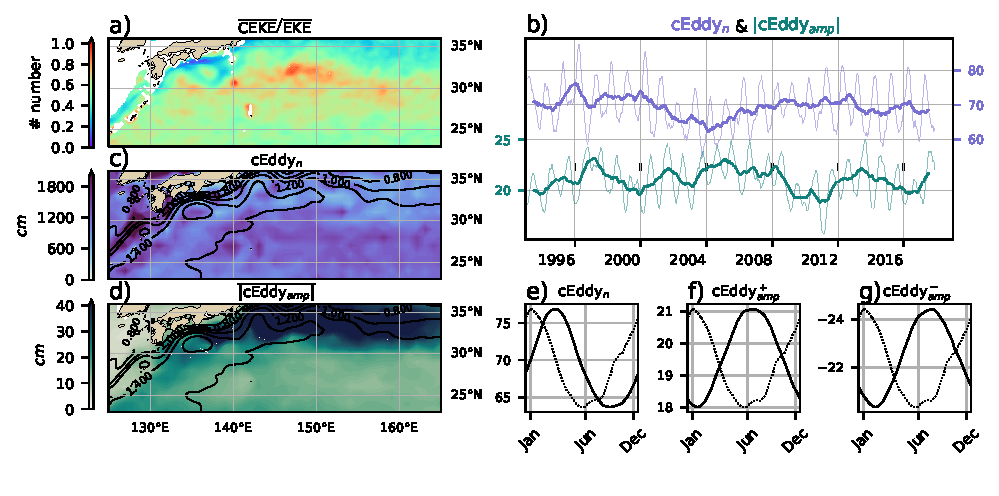
\includegraphics[width=1\textwidth]{figures/regional_ratios_and_stats_V3_4.pdf}
	    \caption{\DIFdelbeginFL \DIFdelFL{Climatology }\DIFdelendFL \DIFaddbeginFL \DIFaddFL{As in Figure \ref{fig:Gulf_Stream}, climatology }\DIFaddendFL of the eddy field and coherent eddy field \DIFdelbeginFL \DIFdelFL{at }\DIFdelendFL \DIFaddbeginFL \DIFaddFL{in }\DIFaddendFL the Kuroshio extension. a) Ratio of mean coherent eddy kinetic energy ($\MCEKE$) versus mean eddy kinetic energy ($\MEKE$); b) Time-series of the coherent eddy number and the average coherent eddy amplitude; c) Map of the number of eddies; d) Map of the average coherent eddy amplitude; Seasonal cycle of the e) number of eddies\DIFdelbeginFL \DIFdelFL{, }\DIFdelendFL \DIFaddbeginFL \DIFaddFL{; }\DIFaddendFL f) positive coherent eddy amplitude, and g) negative coherent eddy amplitude.\DIFdelbeginFL \DIFdelFL{Different lines represent the same as in Figure \ref{fig:Gulf_Stream}.}\DIFdelendFL }
	    \label{fig:Kuroshio}
	\end{figure}

	In the Southern Hemisphere \DIFdelbegin \DIFdel{, }\DIFdelend the strongest boundary current, the Agulhas Current\DIFaddbegin \DIFadd{, }\DIFaddend shows similar behavior to its counterparts in the Northern Hemisphere (Figure \ref{fig:Agulhas}). On average, coherent eddies in the Agulhas \DIFdelbegin \DIFdel{current }\DIFdelend \DIFaddbegin \DIFadd{Current }\DIFaddend contain $\sim$56\% of the energy, meanwhile the $\cEddy_{n}$ seasonal peak occurs in August, while the $\left<|\cEddy_{amp}|\right>$ \DIFaddbegin \DIFadd{peak }\DIFaddend occurs in January-February. 
	The seasonal lag between the winds, eddy count, and eddy amplitude in each of the \DIFdelbegin \DIFdel{western boundary current extensions }\DIFdelend \DIFaddbegin \DIFadd{WBCe }\DIFaddend is interpreted as being analogous to the \DIFdelbegin \DIFdel{explanation observed in Figure \ref{fig:eddy_stats} of the }\DIFdelend lagged response of coherent eddy properties \DIFaddbegin \DIFadd{(Figure \ref{fig:eddy_stats}) }\DIFaddend due to eddy-eddy interactions, consistent with the inverse cascade of energy.

	\begin{figure}
	    \centering
	    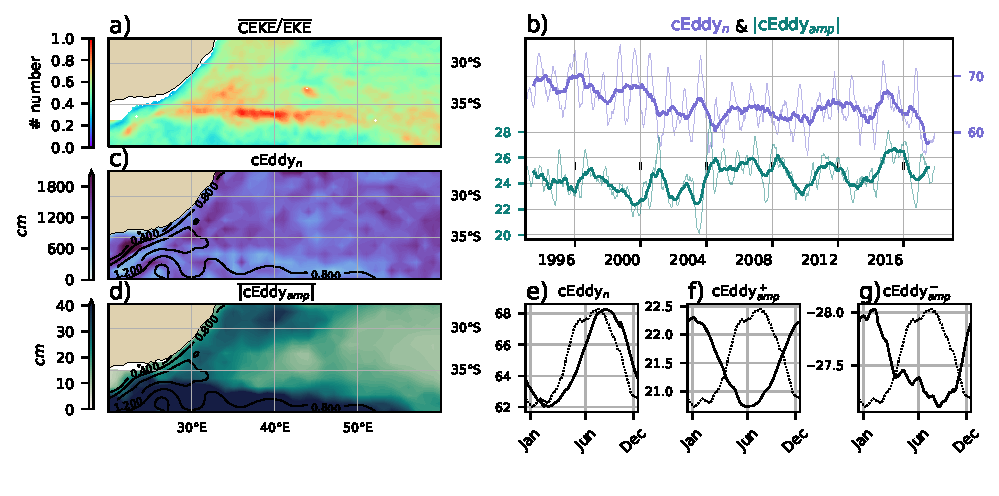
\includegraphics[width=1\textwidth]{figures/regional_ratios_and_stats_V3_2.pdf}
	    \caption{\DIFaddbeginFL \DIFaddFL{As in Figure \ref{fig:Gulf_Stream}, }\DIFaddendFL Climatology of the eddy field and coherent eddy field \DIFdelbeginFL \DIFdelFL{at }\DIFdelendFL \DIFaddbeginFL \DIFaddFL{in }\DIFaddendFL the Agulhas Current. a) Ratio of mean coherent eddy kinetic energy ($\MCEKE$) versus mean eddy kinetic energy ($\MEKE$); b) Time-series of the coherent eddy number and the average coherent eddy amplitude; c) Map of the number of eddies; d) Map of the average coherent eddy amplitude; Seasonal cycle of the e) number of eddies\DIFdelbeginFL \DIFdelFL{, }\DIFdelendFL \DIFaddbeginFL \DIFaddFL{; }\DIFaddendFL f) positive coherent eddy amplitude, and g) negative coherent eddy amplitude.\DIFdelbeginFL \DIFdelFL{Different lines represent the same as in Figure \ref{fig:Gulf_Stream}.}\DIFdelendFL }
	    \label{fig:Agulhas}
	\end{figure}


	% \textbf{Say something about the Leeuwin Current}
	Coherent eddies dominate the $\EKE$ field in other regions such as the Leeuwin Current (Figure \ref{fig:leeuwin_cycle}), where \DIFdelbegin \DIFdel{the }\DIFdelend 65\% of the energy is contained by coherent eddies. 
	\DIFdelbegin \DIFdel{Although the }\DIFdelend \DIFaddbegin \DIFadd{The }\DIFaddend Leeuwin region is not characterized by having a large $\EKE$, however, a considerable abundance of eddies and large eddy amplitudes are \DIFdelbegin \DIFdel{observable }\DIFdelend \DIFaddbegin \DIFadd{observed }\DIFaddend in the region. 
	The \DIFdelbegin \DIFdel{series }\DIFdelend \DIFaddbegin \DIFadd{time-series }\DIFaddend reveal a significant increase in the $\left<|\cEddy_{amp}|\right>$, while the $\cEddy_{n}$ has decreased over the last 3 decades\DIFdelbegin \DIFdel{\mbox{%DIFAUXCMD
\citep{}}\hspace{0pt}%DIFAUXCMD
\textcolor{purple}{\textbf{@Andy}, you suggested a reference here, I couldn't find it...}}\DIFdelend . 
	The seasonal cycle shows that the $\cEddy_{n}$ peak occurs \DIFdelbegin \DIFdel{on }\DIFdelend \DIFaddbegin \DIFadd{in }\DIFaddend August, 3 months after the maximum winds (June). 
	Meanwhile, the $\left<\cEddy_{amp}^+\right>$ responds in synchrony to \DIFaddbegin \DIFadd{the }\DIFaddend winds, and the $\left<\cEddy_{amp}^-\right>$ is in phase with the seasonal cycle of the \DIFaddbegin \DIFadd{eddy number (}\DIFaddend $\cEddy_{n}$\DIFdelbegin \DIFdel{. 
 		}\DIFdelend \DIFaddbegin \DIFadd{). 
	Hence, this region contrast the behavior of WBCe, and showcases the spatial variability of the seasonal cycle of coherent eddies.
 		}\DIFaddend 

	% \textbf{Figure 7}
	% \begin{itemize}
	% 	\item South of the Leeuwin Current there is an important dominance fo the coherent eddy field, where it explains around 80\% of the eddy kinetic energy.
	% 	\item Although this region does not have a large $\EKE$, we can observe a considerable amount of eddies across the region, but more importantly the coherent eddy amplitude is particularly large in those regions with coherent eddy dominance. 
	% 	\item The solid lines show an decrease in the number of eddies, but an increase in the eddy amplitude. 
	% 	\item Moreover, the coherent eddy number peaks in August.
	% 	\item Meanwhile coherent eddies with the positive amplitude have a smaller amplitude than the negative, furthermore, the positive eddies peak in Jun and show a interannual modulation, while the negative eddies peak in October. 
	% 	\item Research regional dynamics (Add here why we may expect this response.)
	% \end{itemize}

	\begin{figure}
	    \centering
	    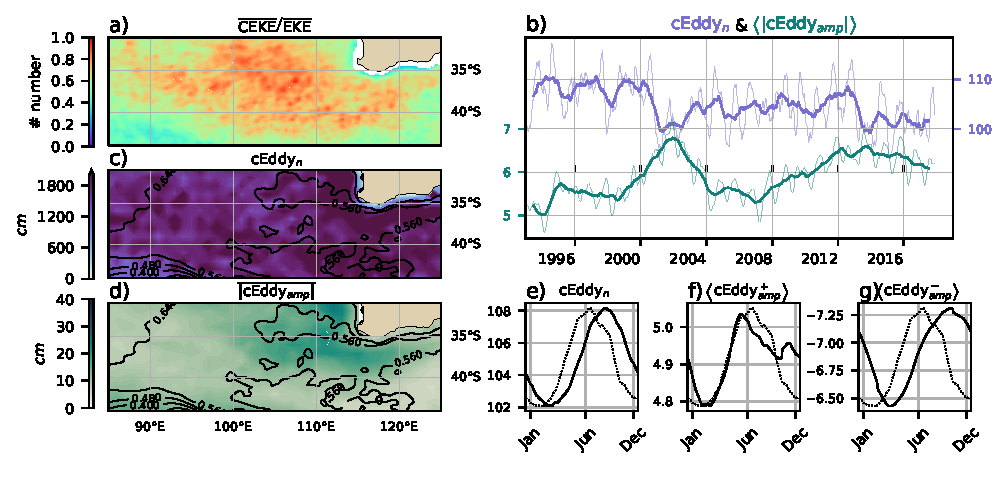
\includegraphics[width=1\textwidth]{figures/regional_ratios_and_stats_V3_0.pdf}
	    \caption{\DIFdelbeginFL \DIFdelFL{Climatology }\DIFdelendFL \DIFaddbeginFL \DIFaddFL{As in Figure \ref{fig:Gulf_Stream}, climatology }\DIFaddendFL of the eddy field and coherent eddy field \DIFdelbeginFL \DIFdelFL{at }\DIFdelendFL \DIFaddbeginFL \DIFaddFL{in }\DIFaddendFL the Leeuwin Current. a) Ratio of mean coherent eddy kinetic energy ($\MCEKE$) versus mean eddy kinetic energy ($\MEKE$); b) Time-series of the coherent eddy number and the average coherent eddy amplitude; c) Map of the number of eddies; d) Map of the average coherent eddy amplitude; Seasonal cycle of the e) number of eddies\DIFdelbeginFL \DIFdelFL{, }\DIFdelendFL \DIFaddbeginFL \DIFaddFL{; }\DIFaddendFL f) positive coherent eddy amplitude, and g) negative coherent eddy amplitude.\DIFdelbeginFL \DIFdelFL{Different lines represent the same as in Figure \ref{fig:Gulf_Stream}.}\DIFdelendFL }
	    \label{fig:leeuwin_cycle}
	\end{figure}

	Another region with important contributions \DIFdelbegin \DIFdel{of }\DIFdelend \DIFaddbegin \DIFadd{to }\DIFaddend the coherent eddy field is the East Tropical Pacific (Tehuantepec region; Figure \ref{fig:tehuantepec}), where coherent eddies contain $\sim$58\% of the energy. 
	In fact, coherent eddy generation in this region is modulated by winds and \DIFdelbegin \DIFdel{coastlly }\DIFdelend \DIFaddbegin \DIFadd{coastally }\DIFaddend trapped waves which produce a strong horizontal and vertical shear (baroclinic and barotropic instabilities; \citealp{Zamudio_Tehuantepec_2006}). 
	Furthermore, the equatorial generated waves propagating along the coast have an important interannual variability observable in the $\left<|\cEddy_{amp}|\right>$ time-series, where El Niño events are notable during 1997 and 2015 (Figure \ref{fig:tehuantepec}b). 
	The seasonal cycle of $\cEddy_{n}$, $\left<\cEddy_{amp}^+\right>$, and $\left<\cEddy_{amp}^-\right>$ support the idea of a coherent \DIFdelbegin \DIFdel{eddies responding }\DIFdelend \DIFaddbegin \DIFadd{eddy response }\DIFaddend to two different coherent eddy generation mechanisms; the number of eddies \DIFdelbegin \DIFdel{seasonal cycle lags for }\DIFdelend \DIFaddbegin \DIFadd{lags }\DIFaddend by $\sim$3 months from the winds, while the $\left<\cEddy_{amp}^+\right>$ is \DIFdelbegin \DIFdel{on }\DIFdelend \DIFaddbegin \DIFadd{in }\DIFaddend phase with the winds and the \DIFdelbegin \DIFdel{maximum of trapped waves }\DIFdelend \DIFaddbegin \DIFadd{time of maximum trapped wave activity }\DIFaddend (winter; \citealp{Zamudio_Tehuantepec_2006}), \DIFdelbegin \DIFdel{and }\DIFdelend \DIFaddbegin \DIFadd{while }\DIFaddend the $\left<\cEddy_{amp}^-\right>$ could be a consequence of eddy-eddy interactions. 

	% \textbf{Figure 9}
	% \begin{itemize}
	% 	\item Here we observe that the number of eddies and eddy amplitude are large in the area where the coherent eddies dominate the eddy field.
	% 	\item Dynamically, in this region eddies are generated due to Rossby wave propagation along the coast that becomes unstable and sheds eddies at the Tehuantepec Gulf.
	% 	\item The seasonal cycle shows a peak in Jun, while the positive amplitude is observed in March and the negative amplitude maximum occurs in September. 
	% 	\item Research regional dynamics (Add here why we may expect this response.)
	% \end{itemize}

	\begin{figure}
	    \centering
	    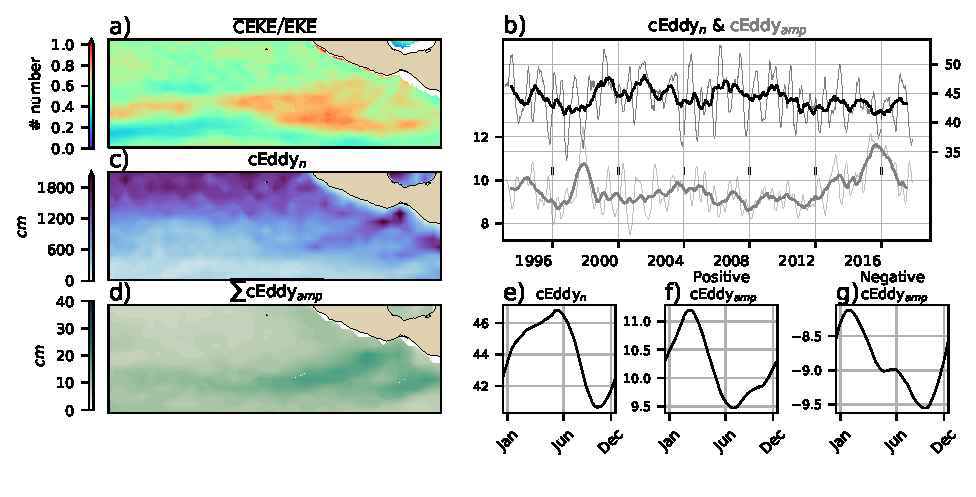
\includegraphics[width=1\textwidth]{figures/regional_ratios_and_stats_V3_3.pdf}
	    \caption{\DIFdelbeginFL \DIFdelFL{Climatology }\DIFdelendFL \DIFaddbeginFL \DIFaddFL{As in Figure \ref{fig:Gulf_Stream}, climatology }\DIFaddendFL of the eddy field and coherent eddy field \DIFdelbeginFL \DIFdelFL{at }\DIFdelendFL \DIFaddbeginFL \DIFaddFL{in }\DIFaddendFL the East Tropical Pacific. a) Ratio of mean coherent eddy kinetic energy ($\MCEKE$) versus mean eddy kinetic energy ($\MEKE$); b) Time-series of the coherent eddy number and the average coherent eddy amplitude; c) Map of the number of eddies; d) Map of the average coherent eddy amplitude; Seasonal cycle of the e) number of eddies\DIFdelbeginFL \DIFdelFL{, }\DIFdelendFL \DIFaddbeginFL \DIFaddFL{; }\DIFaddendFL f) positive coherent eddy amplitude, and g) negative coherent eddy amplitude.\DIFdelbeginFL \DIFdelFL{Different lines represent the same as in Figure \ref{fig:Gulf_Stream}.}\DIFdelendFL }
	    \label{fig:tehuantepec}
	\end{figure}	


	%DIF <  South Australia
	%DIF <  Ratio:  <xarray.DataArray ()>
	%DIF <  array(0.65656905)
	%DIF <  Corr:  [[ 1.         -0.60537253]
	%DIF <  [-0.60537253  1.        ]]
\DIFdelbegin %DIFDELCMD < 

%DIFDELCMD < 	%%%
%DIF <  Agulhas
	%DIF <  Ratio:  <xarray.DataArray ()>
	%DIF <  array(0.56109798)
	%DIF <  Corr:  [[ 1.         -0.27384291]
	%DIF <   [-0.29384291  1.        ]]
%DIFDELCMD < 

%DIFDELCMD < 	%%%
%DIF <  Tehuantepec
	%DIF <  Ratio:  <xarray.DataArray ()>
	%DIF <  array(0.58121928)
	%DIF <  Corr:  [[ 1.         -0.46396017]
	%DIF <  [-0.47396017  1.        ]]
%DIFDELCMD < 

%DIFDELCMD < 	%%%
%DIF <  Kuroshio
	%DIF <  Ratio:  <xarray.DataArray ()>
	%DIF <  array(0.56292827)
	%DIF <  Corr:  [[ 1.         -0.40192595]
	%DIF <   [-0.41192595  1.        ]]
%DIFDELCMD < 

%DIFDELCMD < 	%%%
%DIF <  Gulf stream
	%DIF <  Ratio:  <xarray.DataArray ()>
	%DIF <  array(0.55436168)
	%DIF <  Corr:  [[ 1.         -0.52168401]
	%DIF <  [-0.51168401  1.        ]]
%DIFDELCMD < 

%DIFDELCMD < 	%%%
\DIFdelend % \textbf{Figure 10}
	% \begin{itemize}
	% 	\item Described similar to figure 7, 8, and 9
	% 	\item Note that boundary currents have a consistent seasonal cycle in the positive and negative eddy amplitude.
	% 	\item As expected, the seasonal cycle is opposite to BC in the northern hemisphere.
	% \end{itemize}

	% \textbf{Figure 11}
	% \begin{itemize}
	% 	\item Described similar to figure 7, 8, and 9
	% 	\item Note that boundary currents have a consistent seasonal cycle in the positive and negative eddy amplitude.
	% \end{itemize}

	% \textbf{Figure 12}
	% \begin{itemize}
	% 	\item Described similar to figure 7, 8, and 9
	% 	\item Note that boundary currents have a consistent seasonal cycle in the positive and negative eddy amplitude.
	% 	\item \textcolor{purple}{Delete Fig 11 or 12, they are really similar. What do you think?}
	% \end{itemize}

	% \subsection{Eastern currents}

	% \textbf{Figure 8}
	% \begin{itemize}
	% 	\item South west of the Hawai'i there is an important influence of the coherent eddies.
	% 	\item Although, near we observe a large amount of numbers of eddies in both eddy count form Chelton and JMM, the amplitude is again responsible of the coherent eddy dominance. 
	% 	\item Note the eddy number peaks in March, while the positive eddy amplitude peaks in October, while the negative eddies peak in June.
	% 	\item Research regional dynamics (Add here why we may expect this response.)
	% \end{itemize}

	% \begin{figure}
	%     \centering
	%     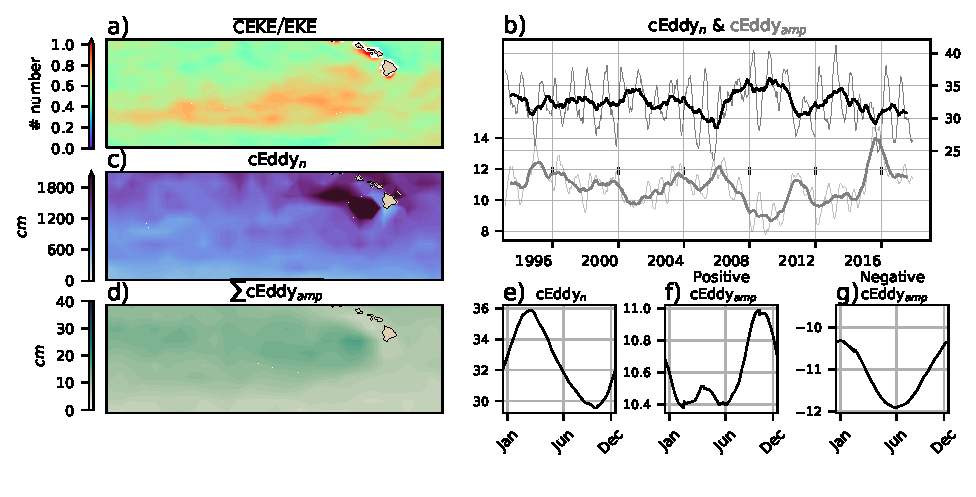
\includegraphics[width=1\textwidth]{figures/regional_ratios_and_stats_V3_1.pdf}
	%     \caption{Same as Figure \ref{fig:leeuwin_cycle} but for the Central North Pacific.}
	%     \label{fig:east_tropical_cycle}
	% \end{figure}

	\section{Discussion and Conclusions}	
	\label{sec:Conclusions}

	We \DIFaddbegin \DIFadd{have }\DIFaddend investigated the contribution of coherent eddies \DIFdelbegin \DIFdel{in the }\DIFdelend \DIFaddbegin \DIFadd{to the total }\DIFaddend kinetic energy field using \DIFaddbegin \DIFadd{available }\DIFaddend satellite observations. 
	We \DIFdelbegin \DIFdel{corroborate }\DIFdelend \DIFaddbegin \DIFadd{found }\DIFaddend that around half of the $\EKE$ is explained by coherent eddies. 
	This half is concentrated in eddy-rich regions where \DIFdelbegin \DIFdel{an }\DIFdelend \DIFaddbegin \DIFadd{a recent multi-decadal }\DIFaddend intensification of the eddy field has been observed \citep{Martinez_Kinetic_2021}. The energy contained by eddies is larger than the previous estimate of 40\% by \citet{Chelton_The_2011}.
	Although there are \DIFdelbegin \DIFdel{difference }\DIFdelend \DIFaddbegin \DIFadd{differences }\DIFaddend in the identification criteria of both eddy identification methods, the main cause of the difference is \DIFdelbegin \DIFdel{believed }\DIFdelend \DIFaddbegin \DIFadd{likely }\DIFaddend to be the lifespan and amplitude filters. 
	These filters are widely used to track individual eddies \DIFdelbegin \DIFdel{on }\DIFdelend \DIFaddbegin \DIFadd{in }\DIFaddend space and time, however, interactions between eddies in energetic regions \DIFdelbegin \DIFdel{my }\DIFdelend \DIFaddbegin \DIFadd{may }\DIFaddend obscure the abundance and influence of short-lived coherent eddies. 
	Filters are not used in this study, and indeed a lack of filters could \DIFdelbegin \DIFdel{facilitates an under or }\DIFdelend \DIFaddbegin \DIFadd{facilitate an }\DIFaddend over-estimation of the the energy contained by coherent eddies, when \DIFdelbegin \DIFdel{miss-identifying or miss-fitting }\DIFdelend \DIFaddbegin \DIFadd{mis-identifying or mis-fitting }\DIFaddend a coherent eddy. \DIFdelbegin \DIFdel{Thus, }\DIFdelend \DIFaddbegin \DIFadd{In hindsight, current generation of climate models have just started to resolve mesoscale dynamics, thus, }\DIFaddend the presented estimate \DIFdelbegin \DIFdel{represents an upper limit of }\DIFdelend \DIFaddbegin \DIFadd{of energy in coherent eddies from satellite observations could be used as a benchmark and quantify }\DIFaddend the energy contained by \DIFdelbegin \DIFdel{coherent eddies}\DIFdelend \DIFaddbegin \DIFadd{mesoscale and more specifically coherent eddies in future climate models}\DIFaddend . 

	\DIFdelbegin \DIFdel{In addition, it should }\DIFdelend \DIFaddbegin \DIFadd{It should also }\DIFaddend be noted that regions with first baroclinic Rossby radius of deformation smaller than 10km cannot be resolved by satellite observations. 
	Thus, the energy contained by coherent eddies around latitudes of 60$^\circ$ and those near the shore are missed from this estimate, and \DIFdelbegin \DIFdel{remains unknown }\DIFdelend their role in the seasonal cycle and local dynamics \DIFaddbegin \DIFadd{remains unknown }\DIFaddend . New satellite altimeter missions (\DIFaddbegin \DIFadd{e.g. Surface Water and Ocean Topography; }\DIFaddend SWOT) may allow \DIFdelbegin \DIFdel{to estimate }\DIFdelend \DIFaddbegin \DIFadd{estimates of the }\DIFaddend energy contained by mesoscale coherent eddies outside the tropical region and the continental slope.

	\DIFdelbegin \DIFdel{Hemispherical }\DIFdelend \DIFaddbegin \DIFadd{Hemisphere-wide }\DIFaddend variability indicates a strong seasonal cycle of the $\EKE$, $\CEKE$, and eddy properties. 
	The seasonal cycle of the $\CEKE$ in each hemisphere occurs as a consequence of numerous small coherent eddies interacting with each other (eddy-eddy interactions) and resulting in stronger, larger and more energetic \DIFaddbegin \DIFadd{(but fewer) }\DIFaddend coherent eddies during summer\DIFaddbegin \DIFadd{, }\DIFaddend after a few months of the yearly coherent eddy number maxima.
	This \DIFdelbegin \DIFdel{results }\DIFdelend \DIFaddbegin \DIFadd{result }\DIFaddend reveals eddy-eddy interactions and thus the transfer of energy from smaller coherent eddies to larger coherent eddies could explain the observed seasonal cycle of $\CEKE$ and coherent eddies properties.

	Coherent eddy properties \DIFdelbegin \DIFdel{showcase }\DIFdelend \DIFaddbegin \DIFadd{reveal }\DIFaddend a non-uniform long-term readjustment of the mesoscale eddy field. 
	Overall, the eddy number has decreased globally at a significant rate of $\sim$35 eddies per decade from $\sim$4000 eddies identified globally on average each day. \DIFdelbegin \DIFdel{However}\DIFdelend \DIFaddbegin \DIFadd{Despite the small changes in the eddy numbers}\DIFaddend , large proportions of the ocean show \DIFdelbegin \DIFdel{an }\DIFdelend \DIFaddbegin \DIFadd{a major }\DIFaddend strengthening of the mesoscale coherent eddy \DIFdelbegin \DIFdel{field at a rate }\DIFdelend \DIFaddbegin \DIFadd{amplitude at rates }\DIFaddend greater than $\sim$1 cm per decade.
	This strengthening of the coherent eddy amplitude is attributed to an intensification of each coherent eddy polarity, rather than a readjustment of the coherent eddy field to sea level rise. 
	In other words, the coherent eddy amplitude intensification is occurring in both coherent eddy polarities and \DIFdelbegin \DIFdel{explain }\DIFdelend \DIFaddbegin \DIFadd{explains }\DIFaddend a proportion of the previously observed readjustments in the eddy field to long-term changes in the ocean forcing \citep{Hu_acceleration_2020,Wunsch_speeding_2020,Martinez_Kinetic_2021}. 
	This long-term readjustment \DIFdelbegin \DIFdel{showcases }\DIFdelend \DIFaddbegin \DIFadd{reveals }\DIFaddend an intensification of the coherent eddy field, possibly due to long-term readjustments in the ocean baroclinic and barotropic instabilities, as well as the strength of the winds.

	The reconstruction of the coherent eddies and their statistics \DIFdelbegin \DIFdel{have }\DIFdelend \DIFaddbegin \DIFadd{has }\DIFaddend revealed regions with important coherent eddy contributions and a distinct seasonal evolution of the coherent eddies. 
	\DIFdelbegin \DIFdel{Remarkably, western boundary extensions }\DIFdelend \DIFaddbegin \DIFadd{Western boundary current extensions (WBCe) }\DIFaddend generate eddies through the instability of the main currents and the seasonal cycle of coherent eddies, $\CEKE$, and thus $\EKE$ could be associated with an inverse energy cascade observable through lagged seasonal cycles in the coherent eddy statistics. 
	In addition\DIFdelbegin \DIFdel{to this}\DIFdelend , the amplitude of the seasonal cycle in \DIFdelbegin \DIFdel{the boundary extensions }\DIFdelend \DIFaddbegin \DIFadd{WBCe }\DIFaddend is two times larger than any other region, thus the seasonality of the coherent eddies in \DIFdelbegin \DIFdel{boundary extensions dominate the hemispherical }\DIFdelend \DIFaddbegin \DIFadd{WBCe dominates the hemispheric }\DIFaddend seasonal cycle. 
	Furthermore, the seasonal lag of the inverse energy cascade is coupled with the presence of fronts \DIFaddbegin \DIFadd{\mbox{%DIFAUXCMD
\citep{Qiu_seasonal_2014}}\hspace{0pt}%DIFAUXCMD
}\DIFaddend , such is the case \DIFdelbegin \DIFdel{of western boundary extensions}\DIFdelend \DIFaddbegin \DIFadd{for WBCe}\DIFaddend , and our results are consistent with the notion of baroclinic instability generating eddies and\DIFdelbegin \DIFdel{through }\DIFdelend \DIFaddbegin \DIFadd{, via }\DIFaddend eddy-eddy interactions\DIFdelbegin \DIFdel{an }\DIFdelend \DIFaddbegin \DIFadd{, a }\DIFaddend lagged inverse energy cascade.

	The use of satellite observations in this study \DIFdelbegin \DIFdel{limit }\DIFdelend \DIFaddbegin \DIFadd{limits }\DIFaddend our ability to quantify the importance of the inverse energy cascade seasonality in the control of the coherent eddy seasonal cycle. 
	As mentioned above, there is robust evidence of an increase in eddy-eddy interactions, however we \DIFdelbegin \DIFdel{can not }\DIFdelend \DIFaddbegin \DIFadd{cannot }\DIFaddend discard important contributions from other processes such as the seasonal cycle of forcing\DIFaddbegin \DIFadd{, stratification, }\DIFaddend and instabilities, which are crucial in the generation of coherent eddies. Although this study can provide a descriptive response of the coherent eddy field, further \DIFdelbegin \DIFdel{studies }\DIFdelend \DIFaddbegin \DIFadd{work is }\DIFaddend are needed to asses the role of eddy-eddy interactions in our changing climate, ocean dynamics, and biogeochemical process. Furthermore, the SWOT mission could allow \DIFaddbegin \DIFadd{us }\DIFaddend to advance our understanding of eddy-eddy interactions and the seasonal cycle of scales smaller than mesoscale, which may provide further evidence of the inverse energy cascade driving the coherent eddy seasonality.

	\acknowledgments
	\DIFaddbegin \DIFadd{The }\DIFaddend \citet{Chelton_mesoscale_2013} dataset was produced by SSALTO/DUACS and distributed by AVISO+ (\url{https://www.aviso.altimetry.fr/}) with support from CNES, developed and validated in collaboration with E.Mason at IMEDEA.
	Global coherent eddy reconstruction, coherent and \DIFdelbegin \DIFdel{non-conherent }\DIFdelend \DIFaddbegin \DIFadd{non-coherent }\DIFaddend eddy kinetic energy datasets, in addition to gridded coherent eddy tracking datasets are publicly available at (\url{https://doi.org/10.5281/zenodo.4646429}).
	All analyses and figures in this manuscript are reproducible via Jupyter notebooks and instructions can be found in the Github repository \texttt{CEKE\_climatology} (\url{https://github.com/josuemtzmo/CEKE_climatology}). Trends used the Python Package xarrayMannKendall (\url{https://doi.org/10.5281/zenodo.4458776})\DIFaddbegin \DIFadd{. J.M.-M. was supported by the Consejo Nacional de Ciencia y Tecnolog\'ia (CONACYT), Mexico funding. M.H.E. is supported by the Centre for Southern Hemisphere Oceans Research (CSHOR), a joint research centre between Qingdao National Laboratory for Marine Science and Technology (QNLM), Commonwealth Scientific and Industrial Research Organisation (CSIRO), University of New South Wales (UNSW), and the University of Tasmania (UTAS).  Analyses were undertaken on the National Computational Infrastructure in Canberra, Australia, which is supported by the Australian Commonwealth Government. 
	}\DIFaddend 

	\bibliography{biblio.bib}

\end{document}
